\documentclass[12pt, a4paper]{article}

% ----- Packages -----
\usepackage[utf8]{inputenc}
\usepackage[T1]{fontenc}
\usepackage[english]{babel}
\usepackage{geometry}
\geometry{margin=2.5cm, headheight=14pt}
\usepackage{graphicx}
\usepackage{float}
\usepackage{hyperref}
\usepackage{xcolor}
\usepackage{enumitem}
\usepackage{setspace}
\usepackage{titlesec}
\usepackage{fancyhdr}
\usepackage{booktabs}
\usepackage{amsmath}
\usepackage{amssymb}
\usepackage{parskip}
\usepackage{caption}
\usepackage{natbib}

% ----- Configuration -----
\hypersetup{
    colorlinks=true,
    linkcolor=blue!60!black,
    citecolor=blue!60!black,
    urlcolor=blue!60!black
}

\onehalfspacing

\pagestyle{fancy}
\fancyhf{}
\fancyhead[L]{\small\leftmark}
\fancyhead[R]{\small\thepage}
\fancyfoot[C]{}
\renewcommand{\headrulewidth}{0.4pt}

\titleformat{\section}{\Large\bfseries}{\thesection.}{0.5em}{}
\titleformat{\subsection}{\large\bfseries}{\thesubsection.}{0.5em}{}
\titleformat{\subsubsection}{\normalsize\bfseries}{\thesubsubsection.}{0.5em}{}

% Titled boxes (title band + tinted background)
\newsavebox{\encadrebox}
\newenvironment{encadre}[1]{%
  \par\bigskip
  \def\encadretitre{#1}%
  \begin{lrbox}{\encadrebox}%
  \begin{minipage}{\dimexpr\linewidth-2\fboxsep-2\fboxrule\relax}%
  \setlength{\parskip}{6pt}%
}{%
  \end{minipage}%
  \end{lrbox}%
  \noindent
  \fcolorbox{blue!50!black}{blue!50!black}{%
    \begin{minipage}{\dimexpr\linewidth-2\fboxsep-2\fboxrule\relax}%
    \textcolor{white}{\textbf{\encadretitre}}%
    \end{minipage}}\par\nointerlineskip
  \noindent
  \fcolorbox{blue!50!black}{blue!5!white}{\usebox{\encadrebox}}%
  \par\bigskip
}

% Figure path
\graphicspath{{output/plots_WD/}{output/plots/}{./}}

% ----- Document -----
\begin{document}

% ========================================
% TITLE PAGE
% ========================================
\begin{titlepage}
\centering
\vspace*{1cm}

{\LARGE\bfseries Macroeconomic effects of the low-carbon transition\\
in developing countries:\\
a comparative analysis of Tunisia and Mexico\\
using the ThreeME model\par}

\vspace{1cm}

{\normalsize\itshape Anonymized manuscript. Author details are provided in the separate title page file.\par}

\vspace{1.5cm}

\textbf{Abstract.} This paper provides a quantitative assessment of the macroeconomic and environmental effects of national low-carbon strategies (NLCS) in two developing economies with opposite energy profiles: Tunisia, a net importer of fossil fuels, and Mexico, a net exporter. Using the neo-Keynesian computable general equilibrium model ThreeME, we simulate ambitious energy transition scenarios up to 2050, combining carbon taxation, the phase-out of fossil fuel subsidies and the deployment of renewable energy, with full recycling of fiscal revenues. The results show that these instruments, when combined, reduce CO$_2$ emissions by 50 to 60\% by 2050 while generating an economic double dividend. A structural asymmetry nevertheless emerges: Tunisia benefits from an immediate expansionary effect through the reduction of its external energy bill and green investment, whereas Mexico has to manage a negative supply shock to its extractive sector, leading to a more complex sectoral reallocation. To the best of our knowledge, this study is the first to provide a systematic comparison, based on a computable general equilibrium model, of the macroeconomic impacts of the low-carbon transition between a fossil-fuel-exporting and a fossil-fuel-importing developing country.

\vspace{0.8cm}

\textbf{Keywords:} Low-carbon transition; Computable general equilibrium model; Double dividend; Developing countries; Tunisia; Mexico

\textbf{JEL classification:} Q48, Q52, Q58, O55, C68

\vfill
\end{titlepage}

% ========================================
% HIGHLIGHTS BOX
% ========================================
\begin{encadre}{Highlights}
\begin{itemize}[leftmargin=*]
    \item First comparative assessment, based on a neo-Keynesian CGE model, of the low-carbon transition in a fossil-fuel-importing (Tunisia) and a fossil-fuel-exporting (Mexico) developing country.
    \item Full recycling of carbon tax revenues is a necessary condition for obtaining an economic double dividend.
    \item The transition is an asymmetric shock: an opportunity for energy sovereignty for the importer, an industrial restructuring challenge for the exporter.
    \item Green investment and job creation in low-carbon sectors largely offset the losses in fossil-fuel-intensive sectors, but the underlying sectoral reallocations call for accompanying policies.
\end{itemize}
\end{encadre}

\vspace{1cm}

% ========================================
% POLICY RECOMMENDATIONS
% ========================================
\begin{encadre}{Policy recommendations}

\textbf{Combine carbon pricing with visible and targeted revenue recycling.} Recycling fiscal revenues is essential to avoid a recessionary effect and to strengthen social acceptability. The proceeds of the carbon tax should finance transfers to households, particularly the most vulnerable, as well as targeted reductions in labour or production costs.

\textbf{Tailor the transition strategy to the country's energy structure.} For net energy importers, the transition can reduce external dependence and improve the trade balance: policies should accelerate the deployment of domestic renewable energy. For hydrocarbon exporters, the transition implies a deeper productive transformation, which must be accompanied by an industrial diversification strategy.

\textbf{Support labour market reallocations.} Even when aggregate employment gains materialise, localised sectoral losses are unavoidable. Training, retraining and occupational mobility policies are needed to limit social costs and sustain political support for the transition.
\end{encadre}

\newpage

% ========================================
% 1. INTRODUCTION
% ========================================
\section{Introduction}
\label{sec:introduction}

\subsection{International context and the heterogeneity of the Global South}

The Paris Agreement, adopted in 2015 under the United Nations Framework Convention on Climate Change (UNFCCC), calls on signatory states to implement ambitious climate policies in order to reach carbon neutrality during the second half of the twenty-first century. To keep global warming below 2\,$^{\circ}$C relative to pre-industrial levels, a balance between greenhouse gas (GHG) emissions and their absorption will have to be achieved (UNFCCC, 2015). In a special report published in October 2018, the Intergovernmental Panel on Climate Change (IPCC) showed that limiting warming to 1.5\,$^{\circ}$C, rather than 2\,$^{\circ}$C, would avoid the most severe consequences of climate change. Reaching this target requires a 45\% reduction in global emissions by 2030 relative to 2010 levels, together with global carbon neutrality by 2050 (IPCC, 2018).

In line with Article~4 of the Agreement, governments are encouraged to activate two complementary levers: on the one hand, the Nationally Determined Contributions (NDCs), which set each country's medium-term climate commitments; on the other hand, national low-carbon strategies (NLCS), which aim to establish a consistent long-term climate trajectory covering all economic sectors. These strategies target deep decarbonisation by 2050, aligning national policies with global GHG reduction objectives.

Faced with this climate emergency, governments are called upon to undertake large-scale structural reforms. The energy sector, as the main emitter of GHG worldwide, is central to this transformation. Reforming energy systems quickly and deeply appears to be an essential lever to steer national trajectories towards carbon neutrality (IEA, 2021; IPCC, 2022; Sovacool et al., 2015).

However, while the macroeconomic effects of such strategies have been widely studied for the most economically developed countries, notably France (Callonnec et al., 2025; Hamdi-Cherif et al., 2025), Germany (Böhringer et al., 2021; Lutz et al., 2021), Spain (Böhringer et al., 2019) or the European Union as a whole (Fragkos et al., 2021; Landis et al., 2021), macroeconomic analyses of low-carbon transitions in developing countries remain much scarcer (Lepault \& Lecocq, 2021).

Yet, throughout the history of climate negotiations and successive COPs, a persistent antagonism has opposed the countries of the North and those of the South. The Global South has long presented itself as carrying a single voice vis-à-vis industrialised countries. However, the homogeneity of the Global South as a single entity is questionable: behind this common label coexist markedly different realities, from small island states threatened with disappearance to large emerging economies with considerable economic power, as well as intermediate countries with very diverse development trajectories. As far as the energy transition is concerned, these national specificities fundamentally condition the nature and magnitude of macroeconomic impacts. A fossil-fuel-importing developing country does not face the same challenges as an exporting one: for the former, the transition can represent an opportunity for energy sovereignty and a reduction of the external bill; for the latter, it implies a potentially costly process of industrial restructuring in the medium term.

It is precisely this heterogeneity that we propose to explore in this paper, by examining two representative cases of these contrasting profiles: Tunisia and Mexico.

\subsection{Tunisia and Mexico: two contrasting energy profiles}

Tunisia has the profile of a small open economy, strongly integrated into European value chains. Once a net exporter of oil and gas, it is now heavily dependent on imports to meet its energy needs, with about 48\% of these needs covered by imports in 2022 (World Bank, 2024). Aggravated by the stagnation of domestic production, this dependence constitutes a major macroeconomic risk. In 2022, energy imports accounted for 53.4\% of the trade deficit, further exposing Tunisia to price volatility on international markets (World Bank, 2024). The state maintains a system of massive fossil fuel subsidies (5.3\% of GDP in 2022; World Bank, 2023a), which weighs heavily on public finances.

Moreover, economic growth remains weak, undermined by persistent political instability and the repercussions of the 2020 health crisis (Dridi, 2024; Elbargathi \& Al-Assaf, 2019). The unemployment rate reached 16.4\% in 2023 (World Bank, 2024), limiting the fiscal space available for public investment. The electricity mix remains dominated by natural gas, with renewables struggling to take off (about 2\% of electricity generation in 2022), despite considerable solar and wind potential, estimated at 320\,GW (Khouaja, 2020). In this context, the energy transition offers a strategic opportunity to strengthen the country's energy independence, improve the sustainability of public finances and foster more inclusive development (World Bank, 2023b).

Mexico, by contrast, stands out as a major emerging economy (GDP of USD~1.85 trillion) and the world's thirteenth-largest oil producer. The Mexican economy displays relative robustness, supported by a diversified industrial base (32\% of GDP including construction) and strong trade integration with the United States. The labour market exhibits a low frictional unemployment rate (2.7\% in 2024), although this masks a significant share of informality. The oil rent, channelled through the national company PEMEX, remains a pillar of fiscal revenues, making decarbonisation politically sensitive, with a risk of stranded assets in the energy sector. Mexico also faces a paradox: while exporting crude oil, it remains an importer of refined products and gas. The Mexican challenge is one of reallocation: how to maintain the price competitiveness of its manufacturing industry while internalising the cost of carbon, without triggering major inflationary shocks.

\subsection{Literature review and positioning}

The macroeconomic implications of low-carbon transitions for developing countries have received growing attention in recent years. Magacho et al. (2023), in a paper published in \textit{World Development}, propose a multidimensional framework to assess developing economies' macroeconomic exposure to the low-carbon transition, considering their reliance on carbon-intensive industries as a source of foreign currency, fiscal revenue, employment and wage income. Their work highlights the heterogeneity of developing countries' vulnerability profiles, but does not rely on a structural macroeconomic model to simulate transition scenarios.

On the side of oil-exporting developing countries, Soummane et al. (2019) use IMACLIM-SAU, a CGE model calibrated for Saudi Arabia, to analyse macroeconomic pathways under global mitigation constraints versus domestic energy price reforms, showing that national energy reforms can generate welfare gains even in a context of declining global fossil fuel demand. Using the GEMINI-E3 CGE model, Babonneau et al. (2023) analyse the strategic options of Gulf countries in a global transition to net-zero emissions, showing that these countries face significant welfare losses but can mitigate stranded asset risks through carbon capture technologies and international emissions trading. More recently, Jacques et al. (2025) couple a stock-flow consistent macroeconomic model with an energy system optimisation model, building on the ThreeME framework, to study the energy transition in Colombia, an oil-exporting developing country facing significant economic and financial imbalances due to the prospective loss of fossil fuel export revenues. Karanfil and Omgba (2023) further examine the structural factors explaining why some oil-dependent countries manage to diversify their economies while others do not.

On the side of energy-importing developing countries, the literature is thinner. Zaghdoud (2025) uses a dynamic CGE-OLG model to analyse environmental fiscal policies and the double dividend in Tunisia, finding that a carbon tax may dampen short-term growth but fosters a sustainable energy transition. Belhadj et al. (2022) assess the macroeconomic, distributive and environmental impacts of energy subsidy removal in Tunisia using an input-output model. O'Ryan et al. (2023) apply a dynamic CGE model to evaluate the potential impacts of a carbon tax in Chile. It should be noted that, in Tunisia, work on the low-carbon transition has mostly focused on sectoral and techno-economic approaches, often of the \textit{bottom-up} type (ANME, 2020; Jebali et al., 2017; Mraihi \& Ben Salem, 2019; UNDP, 2021). Integrated quantitative assessments based on a CGE model adapted to the Tunisian economy are, by contrast, still lacking.

\textbf{To the best of our knowledge, there is no macroeconomic study based on a computable general equilibrium model that systematically compares the impact of a low-carbon transition between a fossil-fuel-exporting and a fossil-fuel-importing developing country.} This is the gap we propose to fill by providing a comparative analysis of Tunisia and Mexico using the ThreeME model, a neo-Keynesian CGE framework that captures short- and medium-term macroeconomic dynamics, sectoral adjustments and employment effects.

\subsection{Contribution and outline}

This study relies on the ThreeME model (Callonnec et al., 2025; Malliet et al., 2016), a computable general equilibrium model specifically adapted to the Tunisian and Mexican economies. The model simulates the macroeconomic, sectoral, technological and environmental effects of different policies, while accounting for the country's energy structure and the behaviour of economic agents. Our central argument is that the energy transition is not a symmetric shock: it represents an opportunity for sovereignty and purchasing power gains for importers, but an industrial restructuring challenge for exporters.

The remainder of the paper is structured as follows. Section~\ref{sec:framework} presents the methodological framework, detailing the ThreeME model, the neo-Keynesian setting that allows a double dividend to emerge, and the simulated scenarios. Section~\ref{sec:recycling} is devoted to the role of fiscal revenue recycling, illustrated by the Tunisian case. Section~\ref{sec:comparison} provides the comparative analysis of the results for Tunisia and Mexico, covering aggregate macroeconomic effects, the decomposition of GDP, investment, sectoral energy and emission dynamics, as well as the trade balance and employment. Section~\ref{sec:discussion} discusses the realism of the simulated decoupling and the limitations of the exercise. Finally, Section~\ref{sec:conclusion} concludes by highlighting the main lessons and policy recommendations.

% ========================================
% 2. METHODOLOGICAL FRAMEWORK
% ========================================
\section{Methodological framework: the ThreeME model and the scenarios}
\label{sec:framework}

\subsection{General features of the ThreeME model}
\label{subsec:threeme}

The analysis is carried out with the Tunisian and Mexican versions of ThreeME, an open-source integrated computable general equilibrium model. This macroeconomic and sectoral model was designed to represent the economy of a country or region, and to assess the economic impacts of environmental and energy policies in the medium and long run, at both the aggregate and sectoral levels (Callonnec et al., 2013, 2025). Initially developed to inform the energy-environment-climate debate in France, ThreeME has since been applied to other national contexts: the Netherlands (Bulavskaya \& Reynès, 2018), Indonesia (Malliet et al., 2016), Mexico (Landa et al., 2016) and Tunisia (Hamdi-Cherif et al., 2025).

ThreeME combines several important features:

\begin{itemize}
    \item \textbf{Sectoral disaggregation}, which makes it possible to trace the effects of activity shifting from one industry to another in terms of employment, investment, energy consumption and foreign trade.
    \item \textbf{Energy disaggregation}, which allows a detailed analysis of energy production and consumption behaviour. Sectors can arbitrate between different energy investments: substitution between capital and energy when the relative price of energy rises, and substitution between energy sources. Households can substitute between energy sources, transport modes or types of goods and services.
    \item \textbf{A hybrid structure}, combining \textit{top-down} macroeconomic modelling with \textit{bottom-up} technical modelling of energy consumption. Its level of disaggregation, particularly for the energy sectors, makes it possible to link up with \textit{bottom-up} models such as MedPro in the Tunisian case.
    \item \textbf{A general equilibrium framework}, taking into account the interactions and feedback effects between supply and demand. Demand (consumption, investment) determines supply (production), which in turn determines demand through the income generated by production factors (labour, capital, etc.).
\end{itemize}

\textit{Note: although they share the same theoretical framework, the ThreeME-Tunisia and ThreeME-Mexico models were developed and calibrated independently by different teams. Differences in sectoral structure, parameter calibration and baseline assumptions make a direct comparison of quantitative results delicate. The comparative analysis below therefore focuses mainly on qualitative mechanisms and relative orders of magnitude rather than on absolute values.}

\subsection{The neo-Keynesian framework and the possibility of a double dividend}
\label{subsec:neokeynesian}

ThreeME is a neo-Keynesian model. Compared with standard Walrasian CGE models, which are largely supply-driven, prices do not instantaneously clear supply and demand. The model is dynamic, and prices and quantities adjust slowly. Producers adjust their supply to demand. This has the advantage of allowing market disequilibria, in particular the presence of involuntary unemployment. This framework is better suited to public policy analysis because it provides information on the transition phase of a given policy, and not only on the long run (Callonnec et al., 2016).

This neo-Keynesian setting has important implications for the properties of the model when a carbon tax is implemented. Most theoretical and empirical studies rejecting the existence of a double dividend base their analysis on a Walrasian market-clearing model. Several studies have shown that such a conclusion depends crucially on strong and specific assumptions (Bento \& Jacobsen, 2007; Kahn \& Farmer, 1999).

In Walrasian CGE models, the capital stock is fixed exogenously, which severely limits the possibility of a double dividend because it restricts substitution between energy and capital. By contrast, in neo-Keynesian CGE models the capital stock is endogenous. The interest rate does not adjust the supply of capital to past savings, but is set by the central bank. An increase in investment in one sector does not require a decrease in investment in another sector. This framework allows for a Keynesian multiplier and a virtuous cycle of economic growth, providing an additional mechanism for the existence of a double dividend that is absent from Walrasian CGE models.

\subsection{The simulated scenarios}
\label{subsec:scenarios}

\subsubsection{Tunisia: four policy configurations}

Within the ThreeME-Tunisia framework, six policy simulations, corresponding to four instrument configurations, are compared with a business-as-usual baseline in which no new climate policy is implemented:

\begin{enumerate}[label=(\roman*)]
    \item \textbf{CT (carbon tax)}: the introduction of a carbon tax, simulated with and without revenue recycling.
    \item \textbf{SUB (subsidy removal)}: the phase-out of fossil fuel subsidies, simulated with and without revenue recycling.
    \item \textbf{REN (renewables)}: an increase in the share of renewable electricity up to 80\% in 2050.
    \item \textbf{NLCS (National Low Carbon Strategy)}: the combination of renewable deployment, subsidy removal, carbon taxation and price signals, with full revenue recycling. This scenario corresponds to Tunisia's complete national low-carbon strategy.
\end{enumerate}

The carbon tax trajectory follows a moderate progression from 1.1 to 9~TND/tCO$_2$ by 2030, then a markedly steeper path reaching 372~TND/tCO$_2$ in 2050 (about USD~132), calibrated to divide GHG emissions by five by 2050 relative to 2020 (Hamdi-Cherif et al., 2025).

\subsubsection{Mexico: the ``Hacienda 2'' scenario}

The low-carbon scenario studied for Mexico, called ``Hacienda 2'', relies on several measures: the deployment of renewable sources for electricity generation, an increase in the carbon tax and the introduction of a tradable ETS quota system, with revenues recycled into the economy. Diesel pricing is modified (reduction of the fiscal incentive) as well as electricity pricing (increase for households and the agricultural sector). The penetration of low-carbon energy in the electricity mix reaches 50\% in 2050 (exogenous in the simulation) and the carbon tax reaches USD~135 in 2050 (Landa et al., 2016).

\subsection{Revenue recycling}
\label{subsec:recycling_mechanism}

The recycling of revenues from the carbon tax and from the removal of energy subsidies is considered in both modelling exercises, as it stimulates economic activity and offsets the recessionary effects of higher energy prices (Aubert \& Chiroleu-Assouline, 2019; Callonnec et al., 2016). In the absence of recycling, fiscal revenues are used solely to repay public debt. With recycling, revenues are redistributed: households receive a share that compensates for the disposable income losses caused by the fiscal policy, and firms receive amounts proportional to their wage bill. As shown in the next section, this mechanism plays a crucial role in the macroeconomic outcomes of transition policies.

% ========================================
% 3. THE IMPORTANCE OF REVENUE RECYCLING
% ========================================
\section{The importance of revenue recycling: evidence from the Tunisian case}
\label{sec:recycling}

\subsection{The double dividend: a result conditional on policy design}

The concept of a ``double dividend'', popularised by Pearce (1991), refers to the idea that the introduction of carbon taxation can deliver two simultaneous benefits: a reduction in environmental damage, which follows directly from the incentive effect of the price signal; and a collective economic gain made possible by the appropriate use of the tax proceeds. The literature distinguishes a ``strong'' version of the double dividend, in which the collective gain exceeds the costs induced by carbon taxation, and a ``weak'' version, in which it only partially offsets these costs (Goulder, 2013).

It is worth stressing that the double dividend is not an ex-ante assumption of the modelling exercise: it is an outcome that may or may not materialise, depending on the design of the policy mix (in particular the use made of the revenues) and on the economic context of each country. Theory identifies the conditions under which it can arise; the simulations then make it possible to verify whether these conditions are met. In Walrasian models, the double dividend is generally limited and rests essentially on two mechanisms: a lower fiscal distortion on labour, and an improvement in the trade balance when the tax penalises foreign products more heavily. In the neo-Keynesian framework of ThreeME, an additional mechanism comes into play: the Keynesian multiplier can trigger a virtuous growth cycle (Callonnec et al., 2016; Landa \& Reynès, 2025).

The meta-analysis by Maxim et al. (2019) shows that the effectiveness of historical examples of carbon taxation depends largely on the nature of the instruments used for collection and transfer, and that the optimal policy mix differs across national contexts.

\subsection{The Tunisian example: with and without recycling}

In the Tunisian modelling exercise, the same transition measures are simulated with and without revenue recycling. Comparing these variants makes it possible to observe empirically whether a double dividend emerges.

\begin{figure}[H]
    \centering
    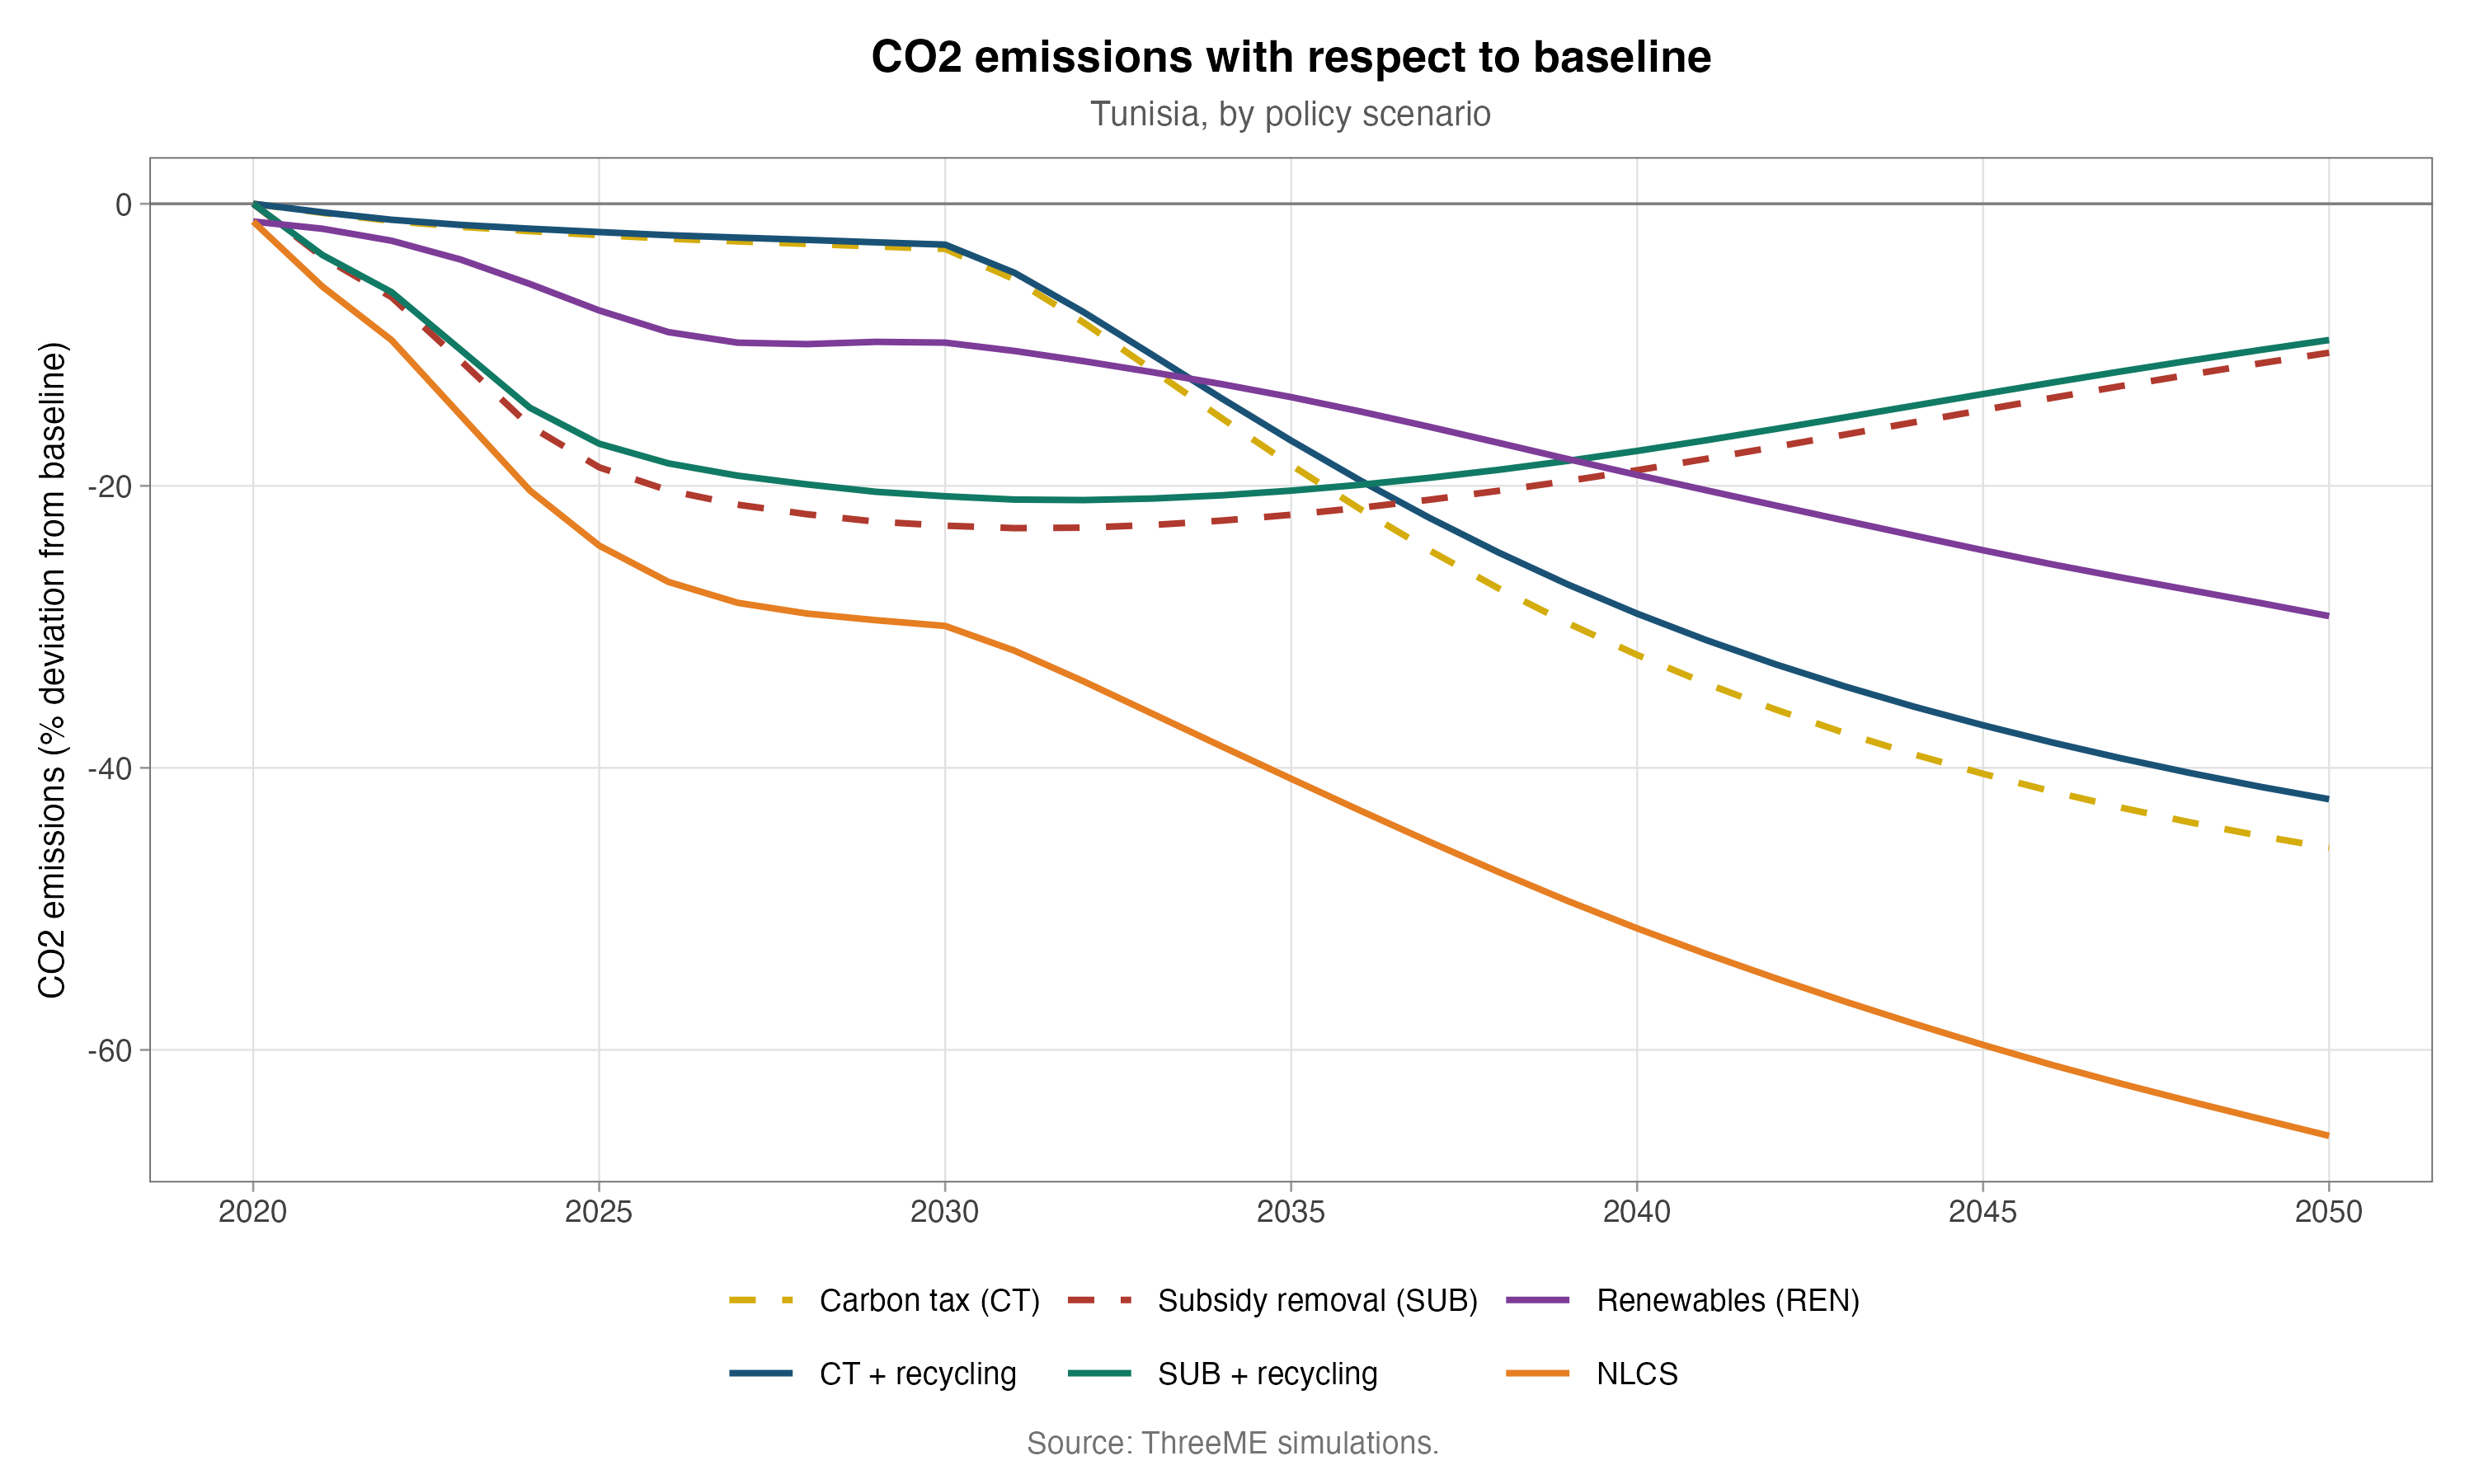
\includegraphics[width=0.95\textwidth]{fig01_co2_scenarios_tunisie.png}
    \caption{CO$_2$ emissions by scenario with respect to baseline in Tunisia, with and without recycling}
    \label{fig:co2_scenarios}
\end{figure}

On the environmental side, the scenarios with and without recycling display comparable emission reductions, albeit slightly larger in the scenarios without recycling, which is explained by lower economic activity (Figure~\ref{fig:co2_scenarios}).

\begin{figure}[H]
    \centering
    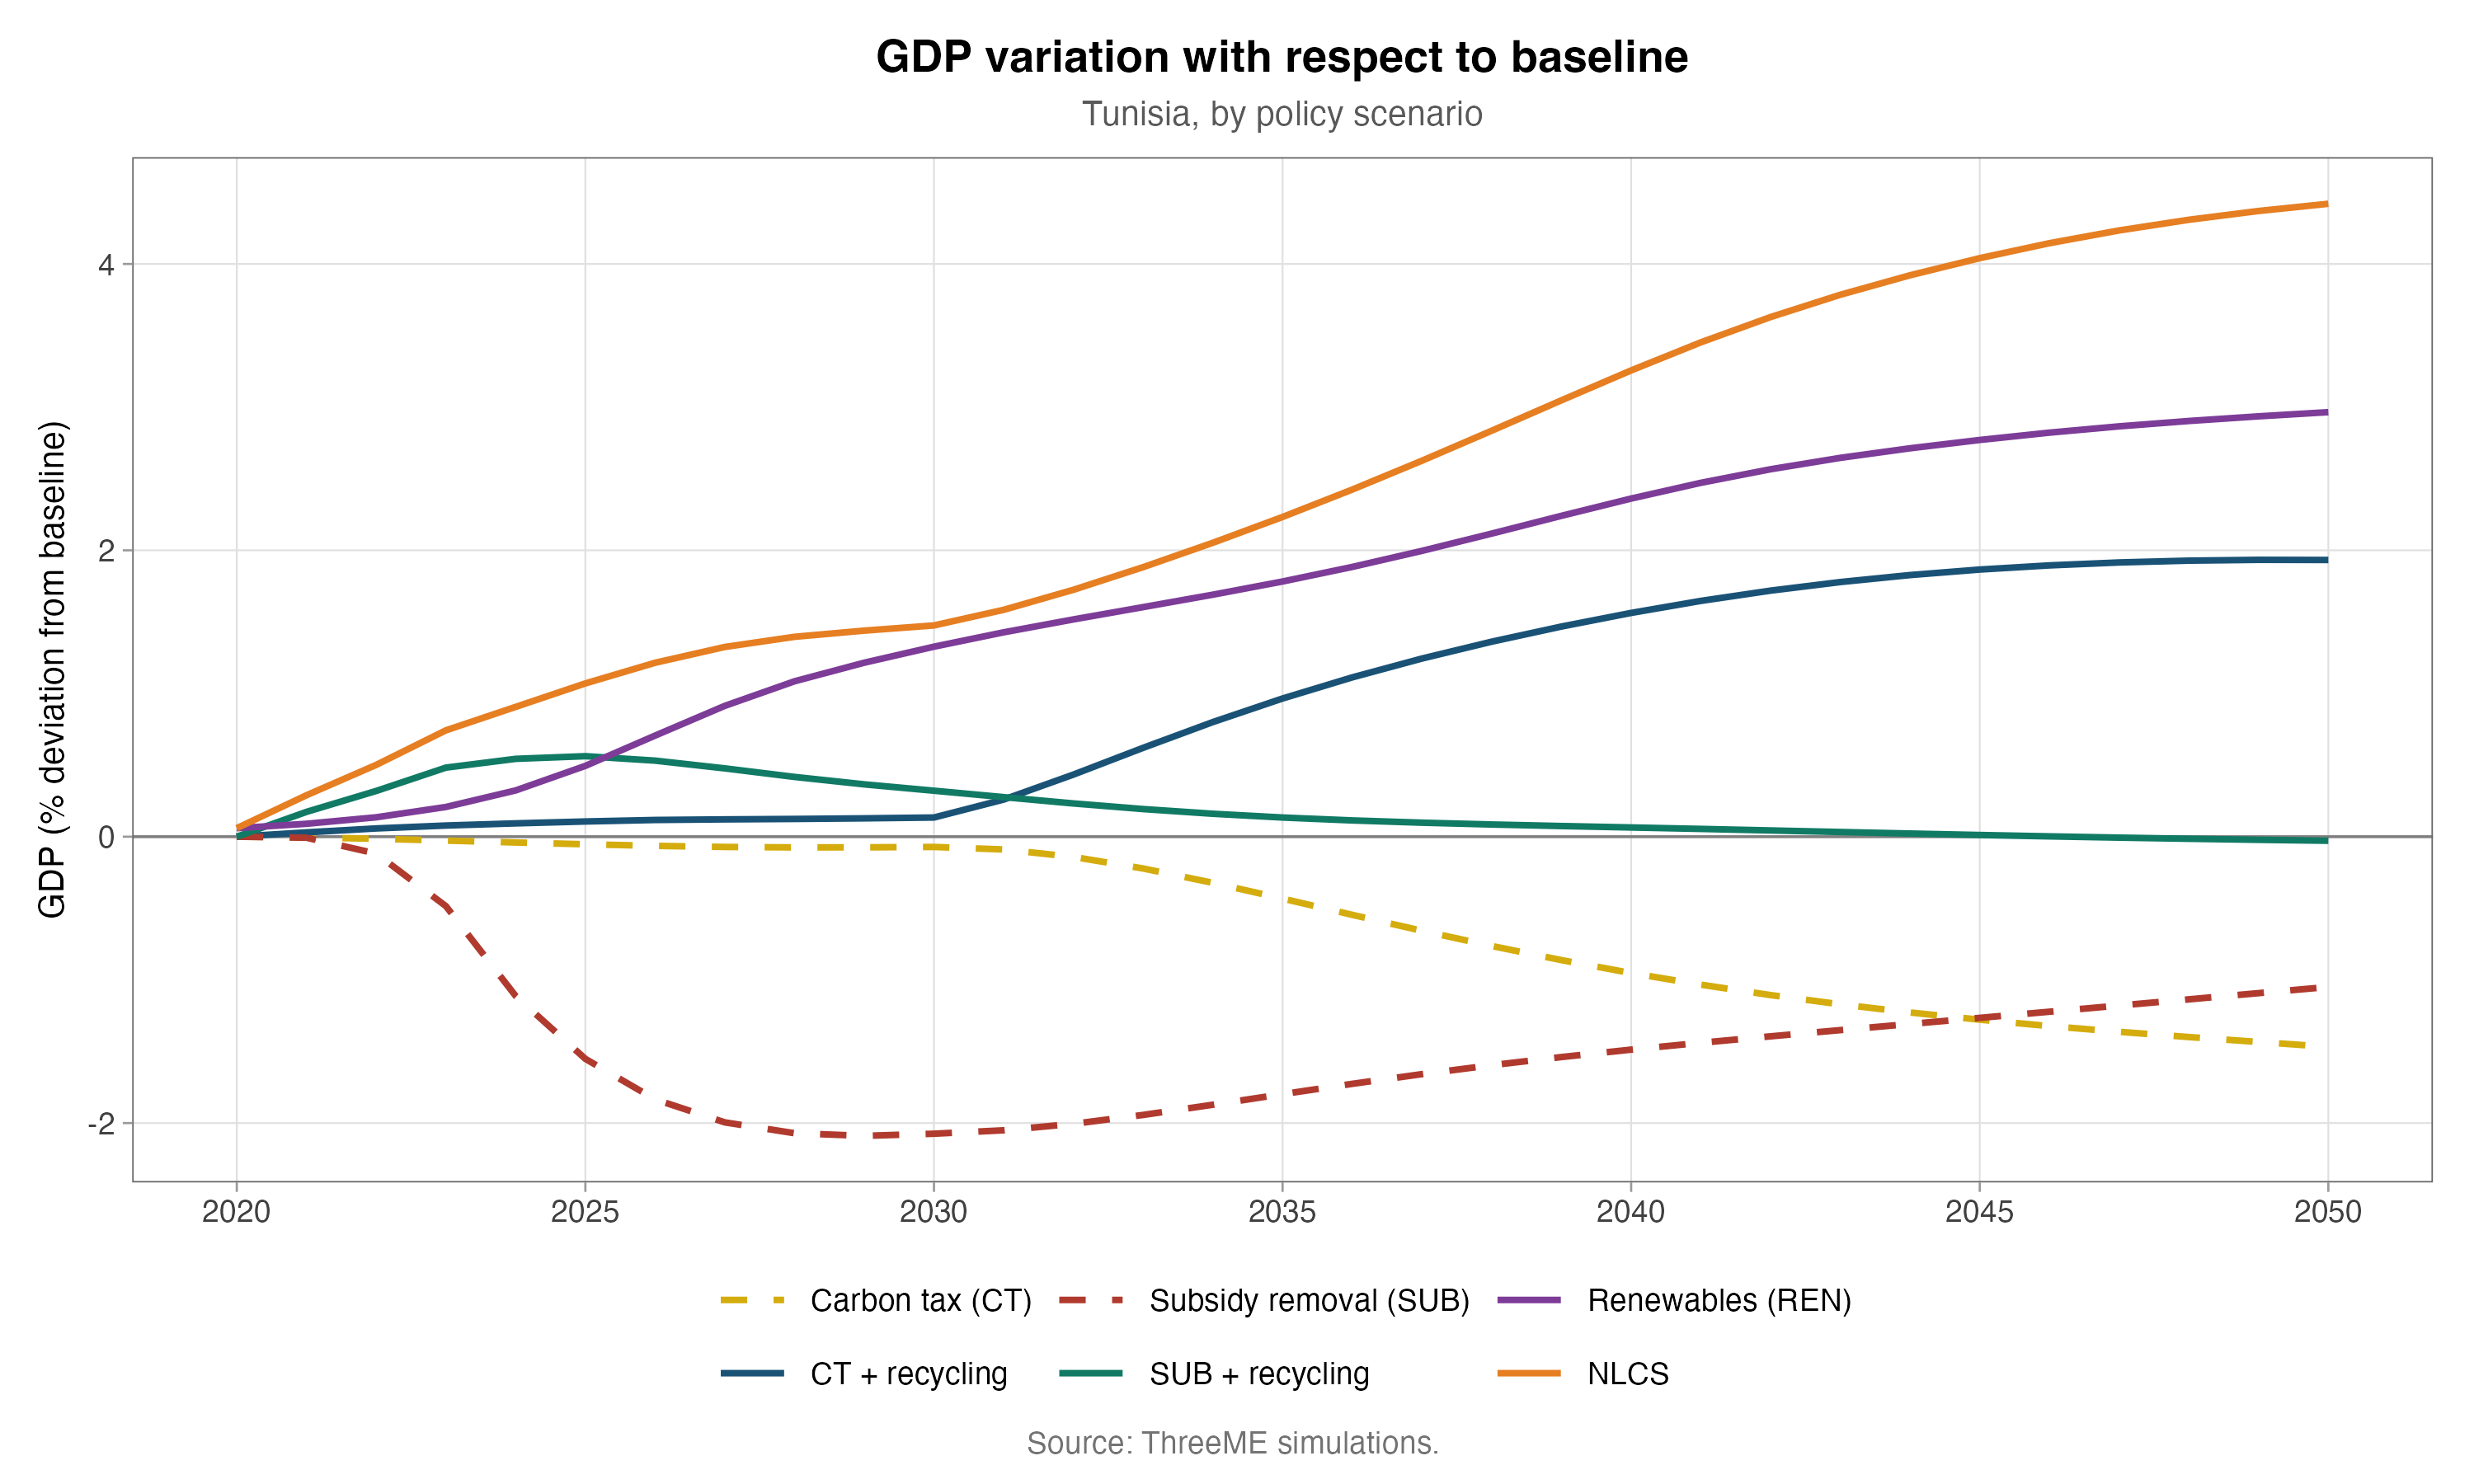
\includegraphics[width=0.95\textwidth]{fig02_pib_scenarios_tunisie.png}
    \caption{GDP variation by scenario with respect to baseline in Tunisia, with and without recycling}
    \label{fig:gdp_scenarios}
\end{figure}

On the economic side, the scenarios with recycling display markedly better macroeconomic indicators than their counterparts without recycling (Figure~\ref{fig:gdp_scenarios}). GDP is below its baseline level in the scenarios without recycling and above it with recycling. The economic dividend of low-carbon fiscal measures thus emerges thanks to recycling. The analysis of aggregate and sectoral impacts confirms that revenue recycling is a necessary condition for obtaining a double dividend in the Tunisian context. The remainder of this paper compares national scenarios with full recycling of carbon revenues.

% ========================================
% 4. COMPARATIVE ANALYSIS TUNISIA-MEXICO
% ========================================
\section{Comparative analysis: the transition in Tunisia and Mexico}
\label{sec:comparison}

In this section, we provide a comparative analysis of the energy transition strategies of Tunisia and Mexico. In both cases, transition policy scenarios for developing countries are simulated with the ThreeME model, in collaboration with local stakeholders, leading to the creation of original national models parameterised with country-specific data.

While the Tunisian and Mexican economies are very different, the simulation exercises display interesting similarities: carbon tax collection reaches a similar level of between 2 and 3 points of GDP in 2050, the carbon price reaches respectively USD~132 and USD~135 per tonne of CO$_2$, and the penetration of renewables in the electricity mix is substantial, at 80\% in Tunisia and 50\% in Mexico.

\subsection{Carbon pricing trajectories}

\begin{figure}[H]
    \centering
    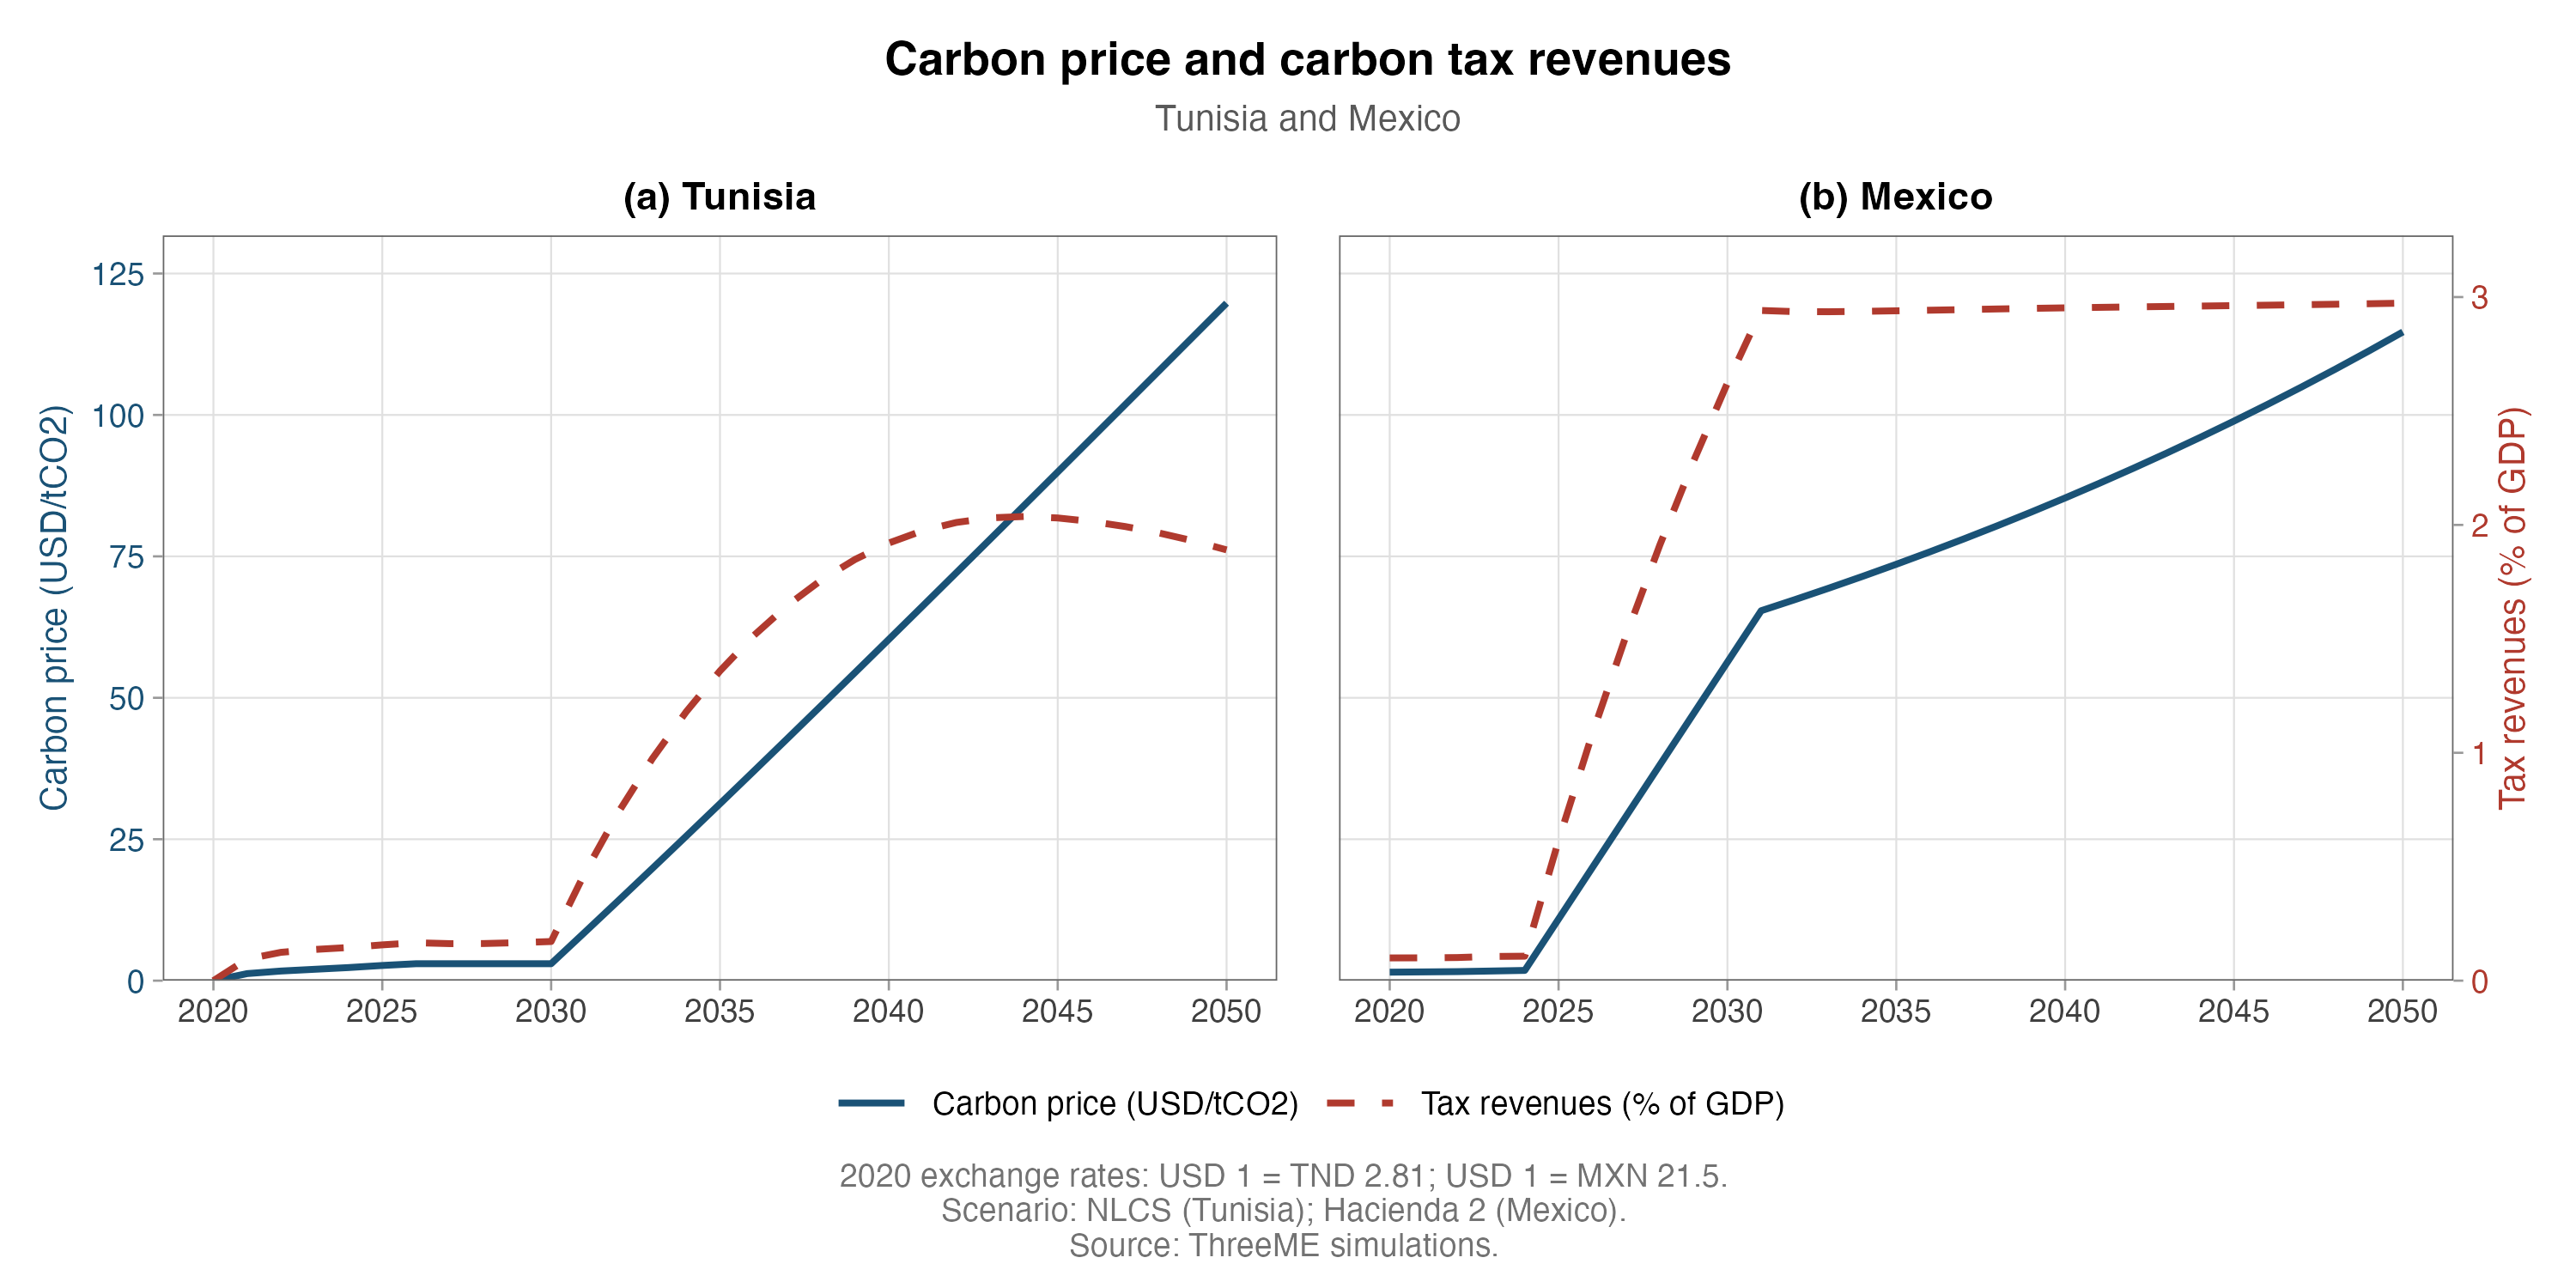
\includegraphics[width=0.95\textwidth]{fig03_taxe_carbone.png}
    \caption{Carbon tax trajectories in Tunisia and Mexico}
    \label{fig:carbon_tax}
\end{figure}

Figure~\ref{fig:carbon_tax} shows that while carbon tax levels are comparable in 2050, the trajectories differ: the carbon tax rises faster in Mexico around 2030, whereas it only reaches a similar level about ten years later in the Tunisian scenario. This difference in pace has important implications for short- and medium-term dynamics, as we will see in the analysis of the results.

\subsection{Environmental effectiveness and decoupling}

The transition strategies achieve their objective in both countries. By 2050, emissions fall by about 60\% in Tunisia and 50\% in Mexico relative to their respective baselines. This decline, combined with higher GDP, produces a decoupling between growth and emissions (Figure~\ref{fig:decoupling}).

\begin{figure}[H]
    \centering
    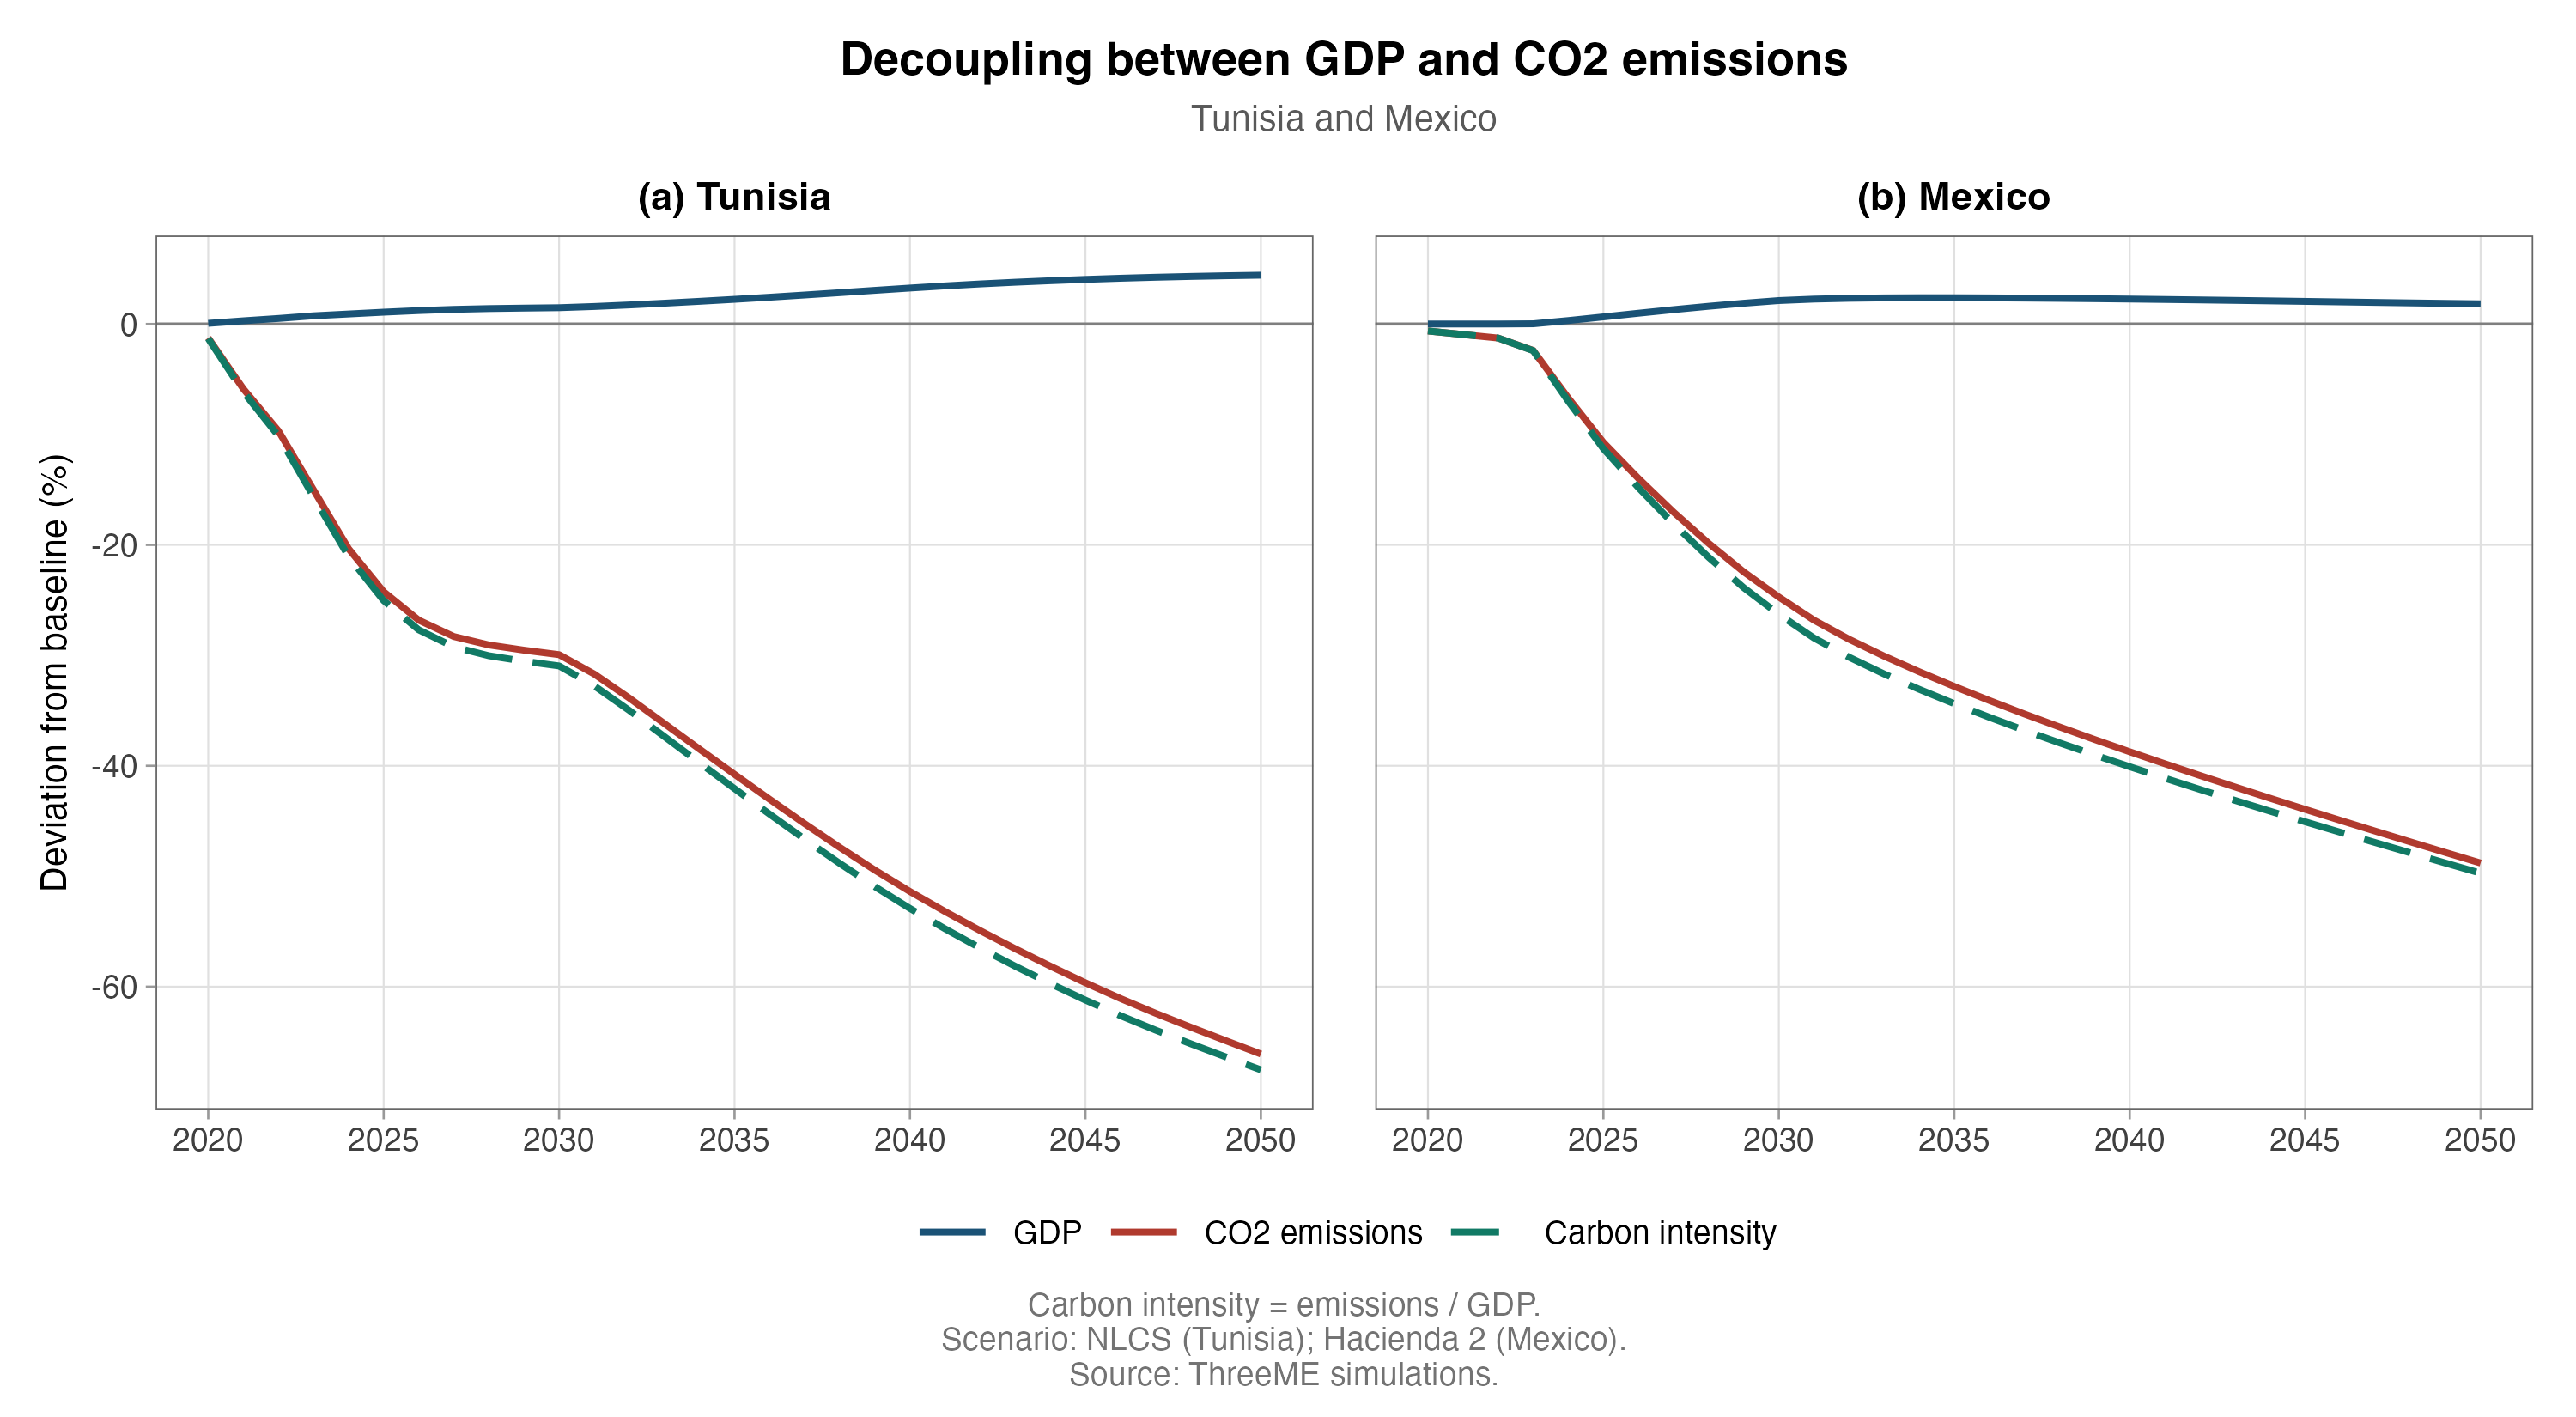
\includegraphics[width=0.95\textwidth]{fig04_decouplage.png}
    \caption{Decoupling between economic growth and CO$_2$ emissions}
    \label{fig:decoupling}
\end{figure}

\subsection{Aggregate macroeconomic effects: an asymmetric shock}

\begin{figure}[H]
    \centering
    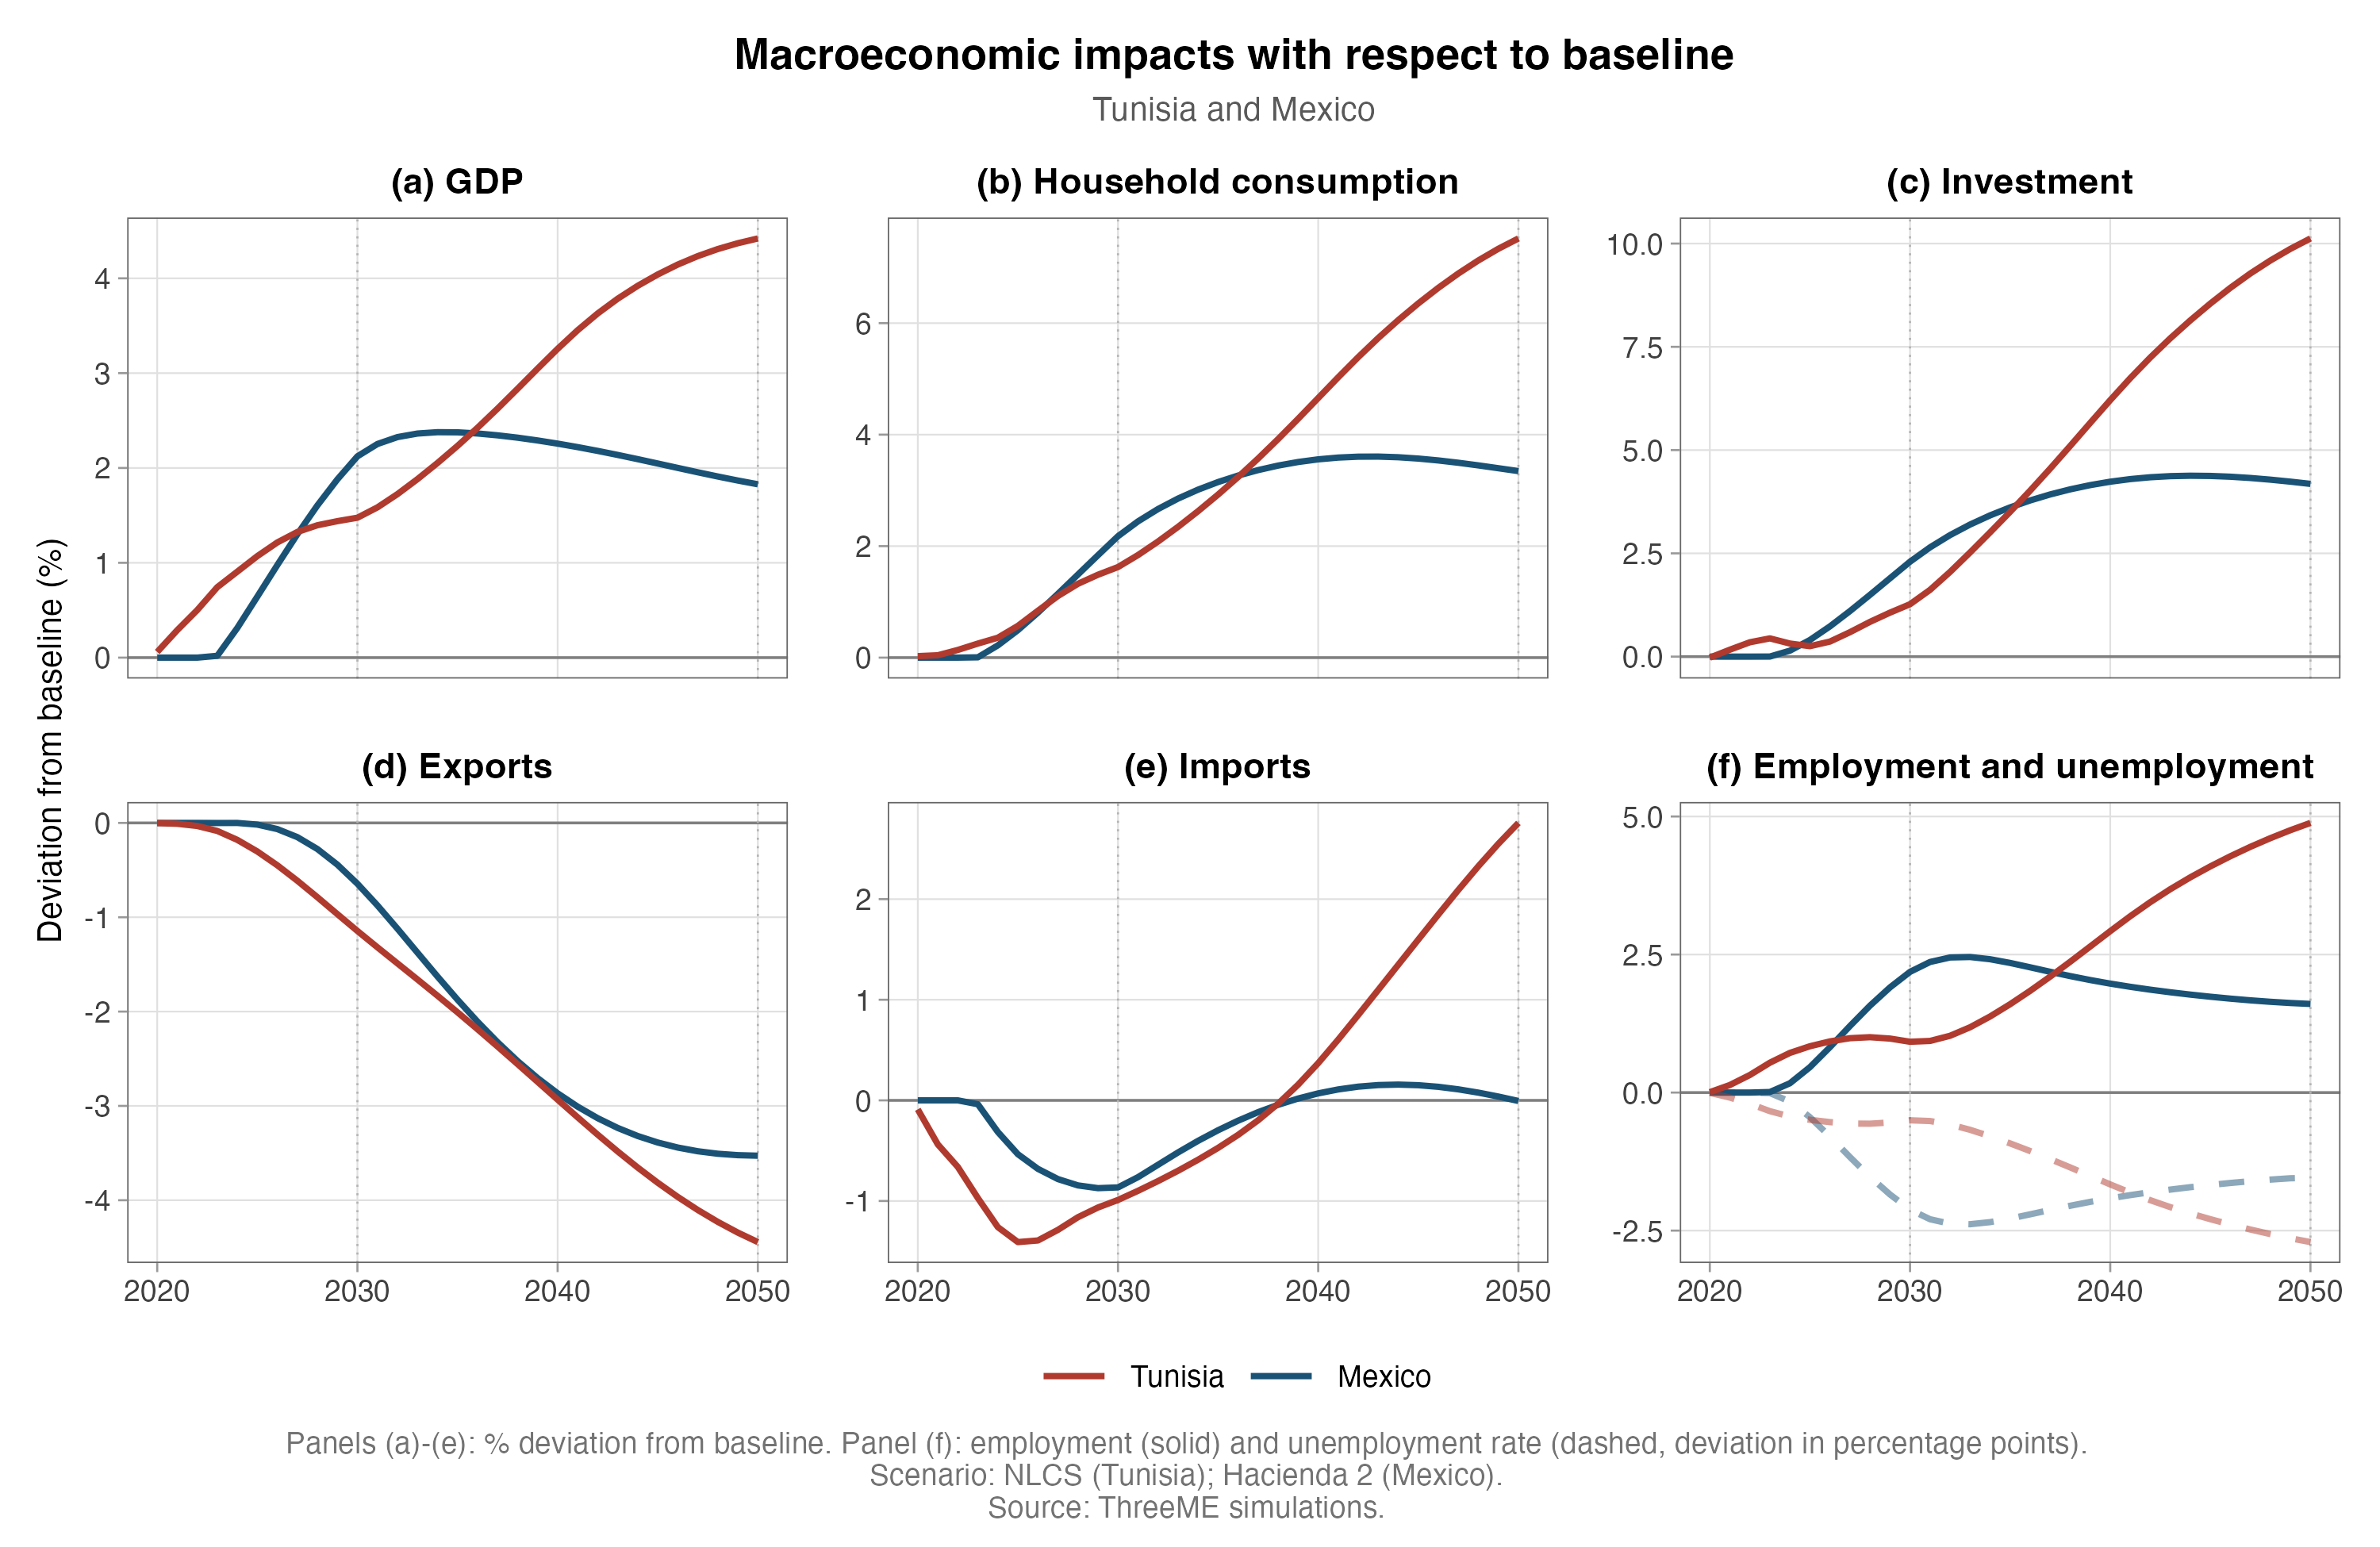
\includegraphics[width=0.95\textwidth]{fig05_impact_macro.png}
    \caption{Macroeconomic impacts with respect to baseline in Tunisia and Mexico}
    \label{fig:macro_impact}
\end{figure}

The comparison of the main macroeconomic indicators (Figure~\ref{fig:macro_impact}) shows that, by 2050, the Tunisian policy mix generates larger gains relative to the baseline than the Mexican one. We explain this with three key arguments.

\textbf{First, the asymmetric nature of the shock depending on the energy structure.} In Tunisia, a net importer of hydrocarbons, carbon pricing and the rise of renewables progressively reduce external energy demand, replaced by domestic electricity generation. The fall in fossil fuel imports improves the trade balance and relocates part of energy spending towards investment and the production of less carbon-intensive sectors. The transition thus acts as a positive demand shock, supported by green investment and the associated multiplier effects: investment in renewable infrastructure operates like a stimulus package.

In Mexico, the transition translates into a negative supply shock to a key exporting sector. The carbon tax leads to a fall in aggregate demand for the energy sector. The competitiveness and profitability of the oil sector decline, leading to a contraction of fossil fuel production and a reallocation of capital and labour towards other sectors. While renewables and services expand, this expansion only gradually offsets the loss of value added in the extractive industry.

\textbf{Second, the importance of the initial macroeconomic situation.} Tunisia, on a sub-optimal growth path marked by high unemployment, has idle production factors. The additional investment and demand associated with the transition resemble a form of green Keynesianism that amplifies the positive effects on GDP, consumption and employment. For Mexico, closer to full employment, the Keynesian multiplier is more strongly constrained by the availability of production factors.

\textbf{Third, the temporal dimension and the price signal.} The faster increase of the tax in Mexico accelerates the relative decline of the oil sector and intensifies the need for sectoral reallocation, weighing more heavily on medium-term macroeconomic dynamics. In Tunisia, the first phase is mainly driven by the effect of investment in renewables, with a gradual increase in the price signal that reinforces the substitution away from fossil fuel imports.

\subsection{GDP decomposition by demand components}
\label{subsec:gdp_decomposition}

To understand the mechanisms underlying GDP dynamics, we analyse the contribution of each component of final demand to the GDP deviation from the baseline (Figure~\ref{fig:gdp_decomp}).

\begin{figure}[H]
    \centering
    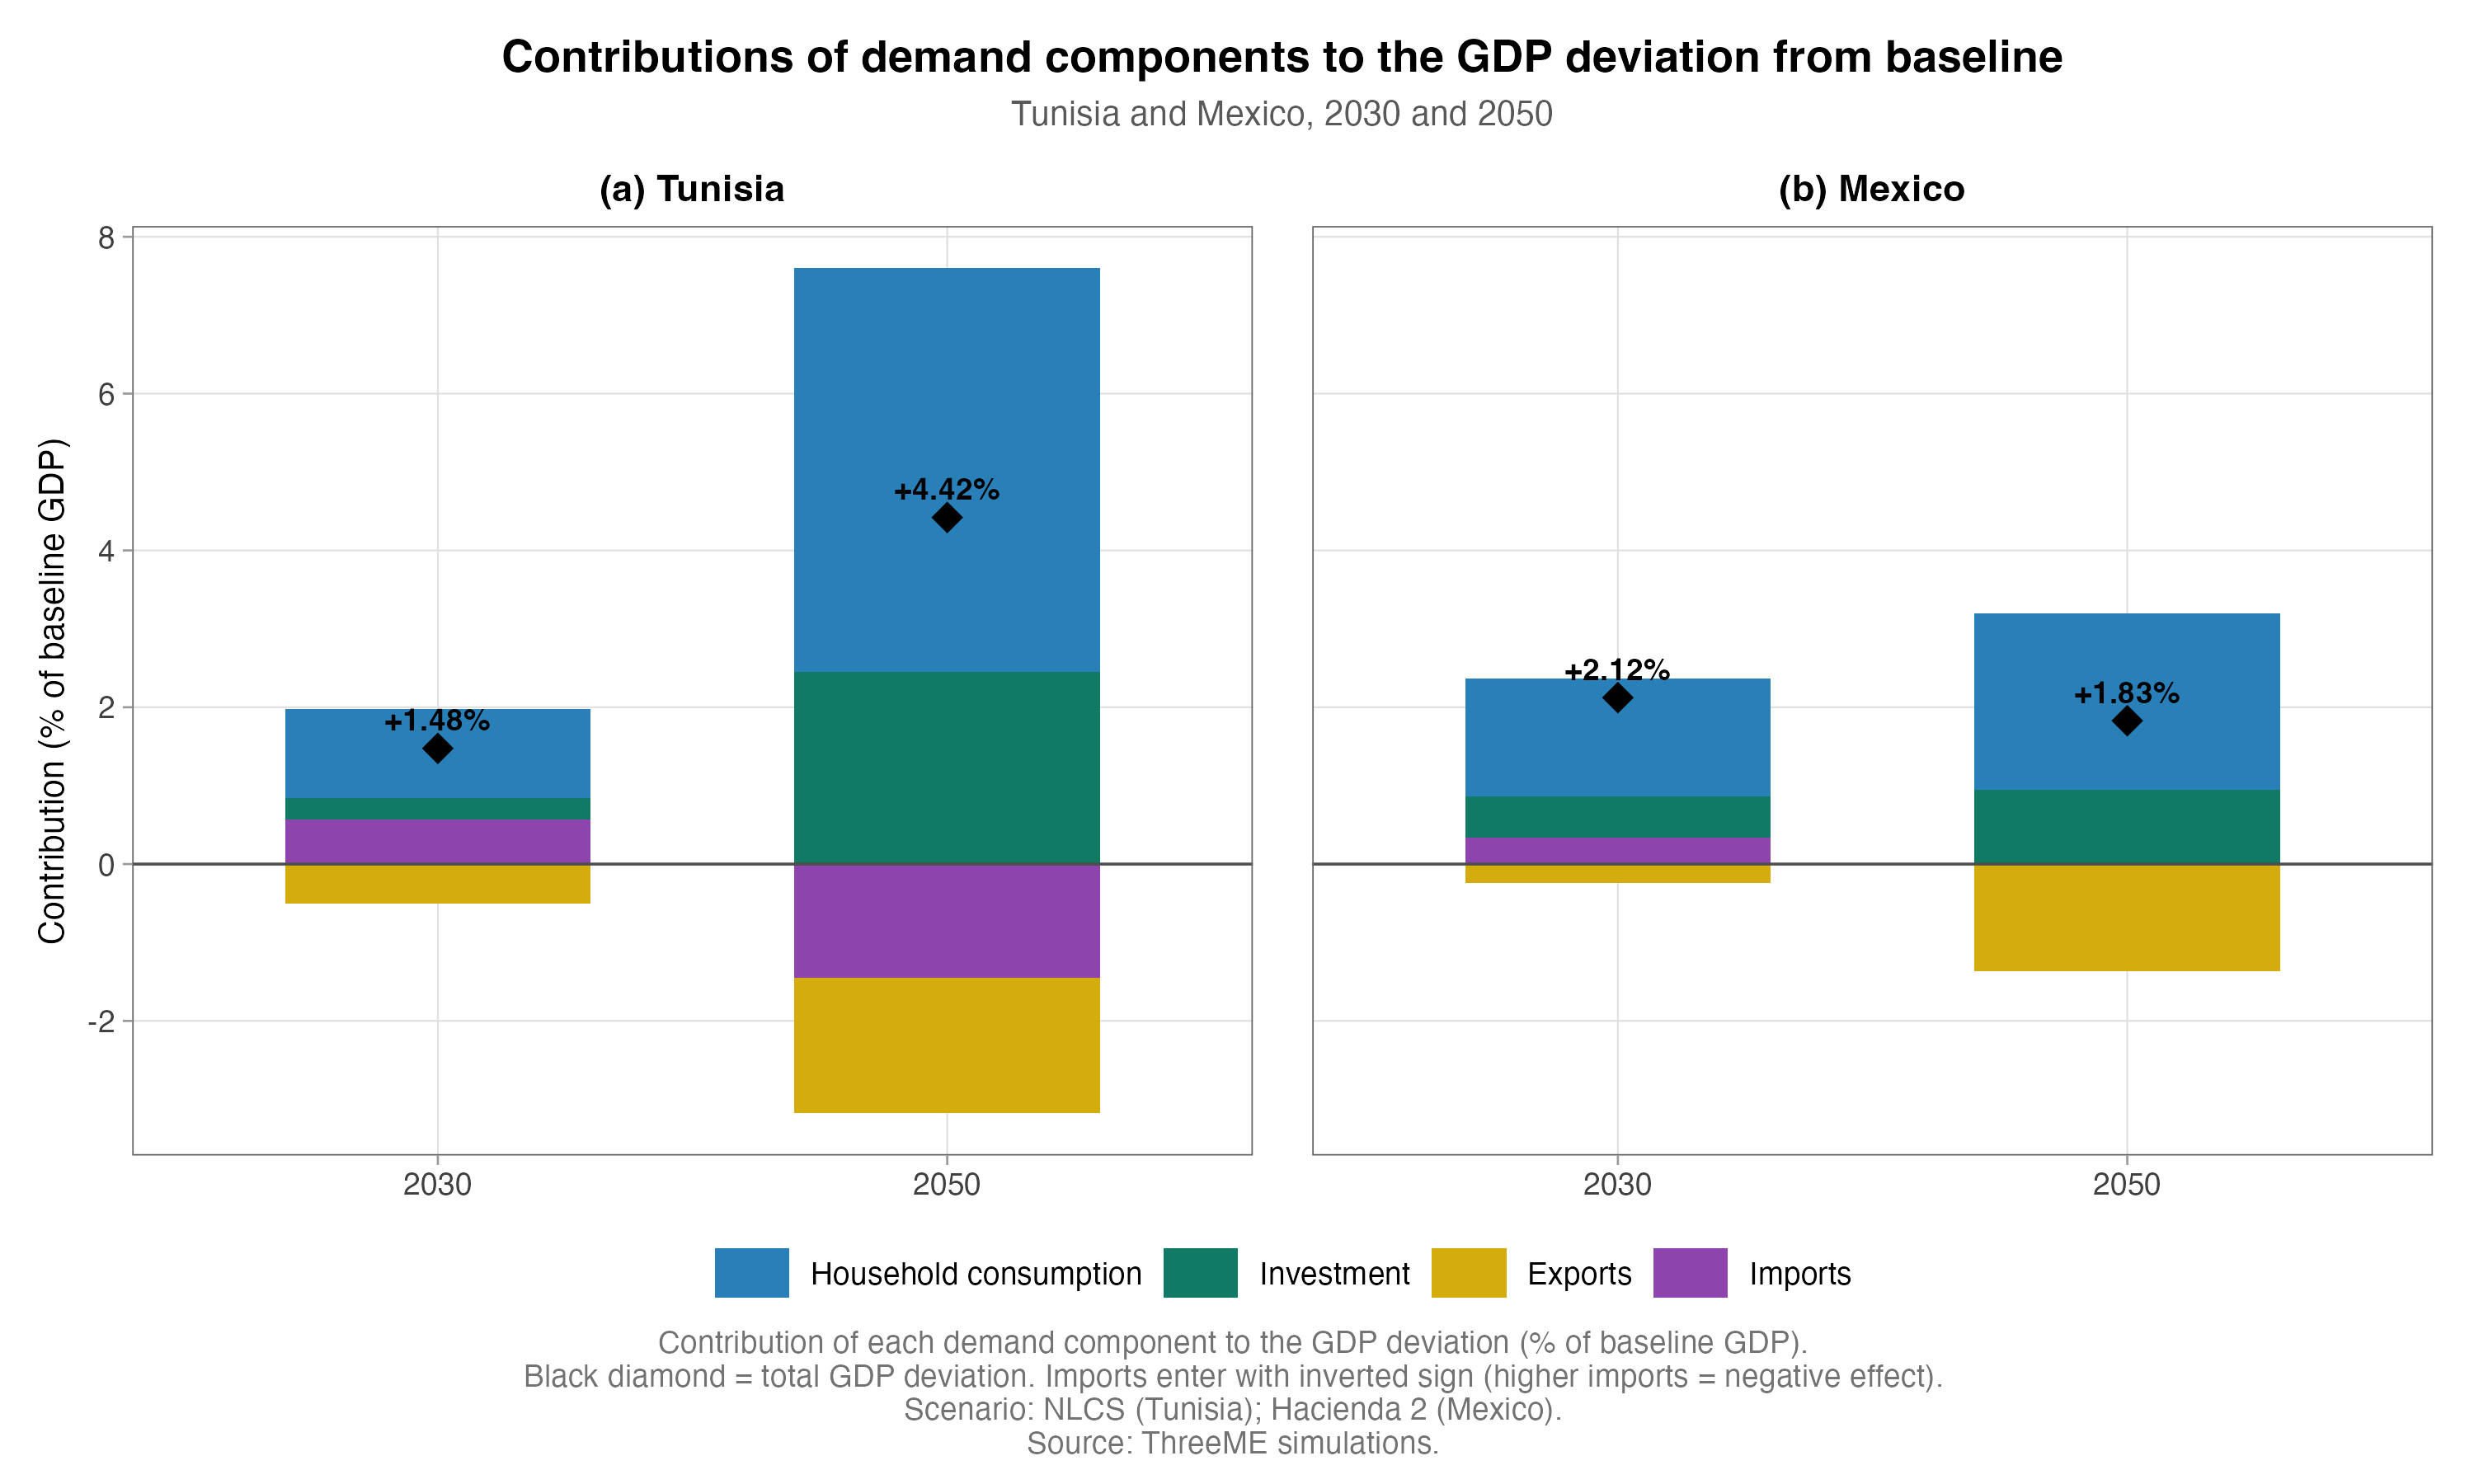
\includegraphics[width=0.95\textwidth]{fig08_decomposition_pib.png}
    \caption{Contributions of demand components to the GDP deviation in Tunisia (NLCS) and Mexico, 2030 and 2050}
    \label{fig:gdp_decomp}
\end{figure}

For Tunisia, in the NLCS scenario, the positive effects clearly dominate. Household consumption and productive investment are the main growth drivers, offsetting the negative contribution of the trade balance. Tunisian GDP rises by 1\% as early as 2025, then by 2.13\% in 2035, reaching +5\% by 2050 relative to the baseline. This sustained progression reflects robust dynamics driven by household consumption and productive investment, which compensate for the external tensions generated by the deterioration of the trade balance.

For Mexico, investment also plays a driving role, but the negative contribution of net exports is more pronounced, reflecting the loss of competitiveness of the fossil fuel sector and the increased need for imported capital goods.

\subsection{Investment dynamics}
\label{subsec:investment}

One of the major macroeconomic effects of the transition concerns investment. As a central engine of the transformation of the productive system, it responds differently depending on the policy instruments implemented, but shows an overall positive dynamic in the long run.

\begin{figure}[H]
    \centering
    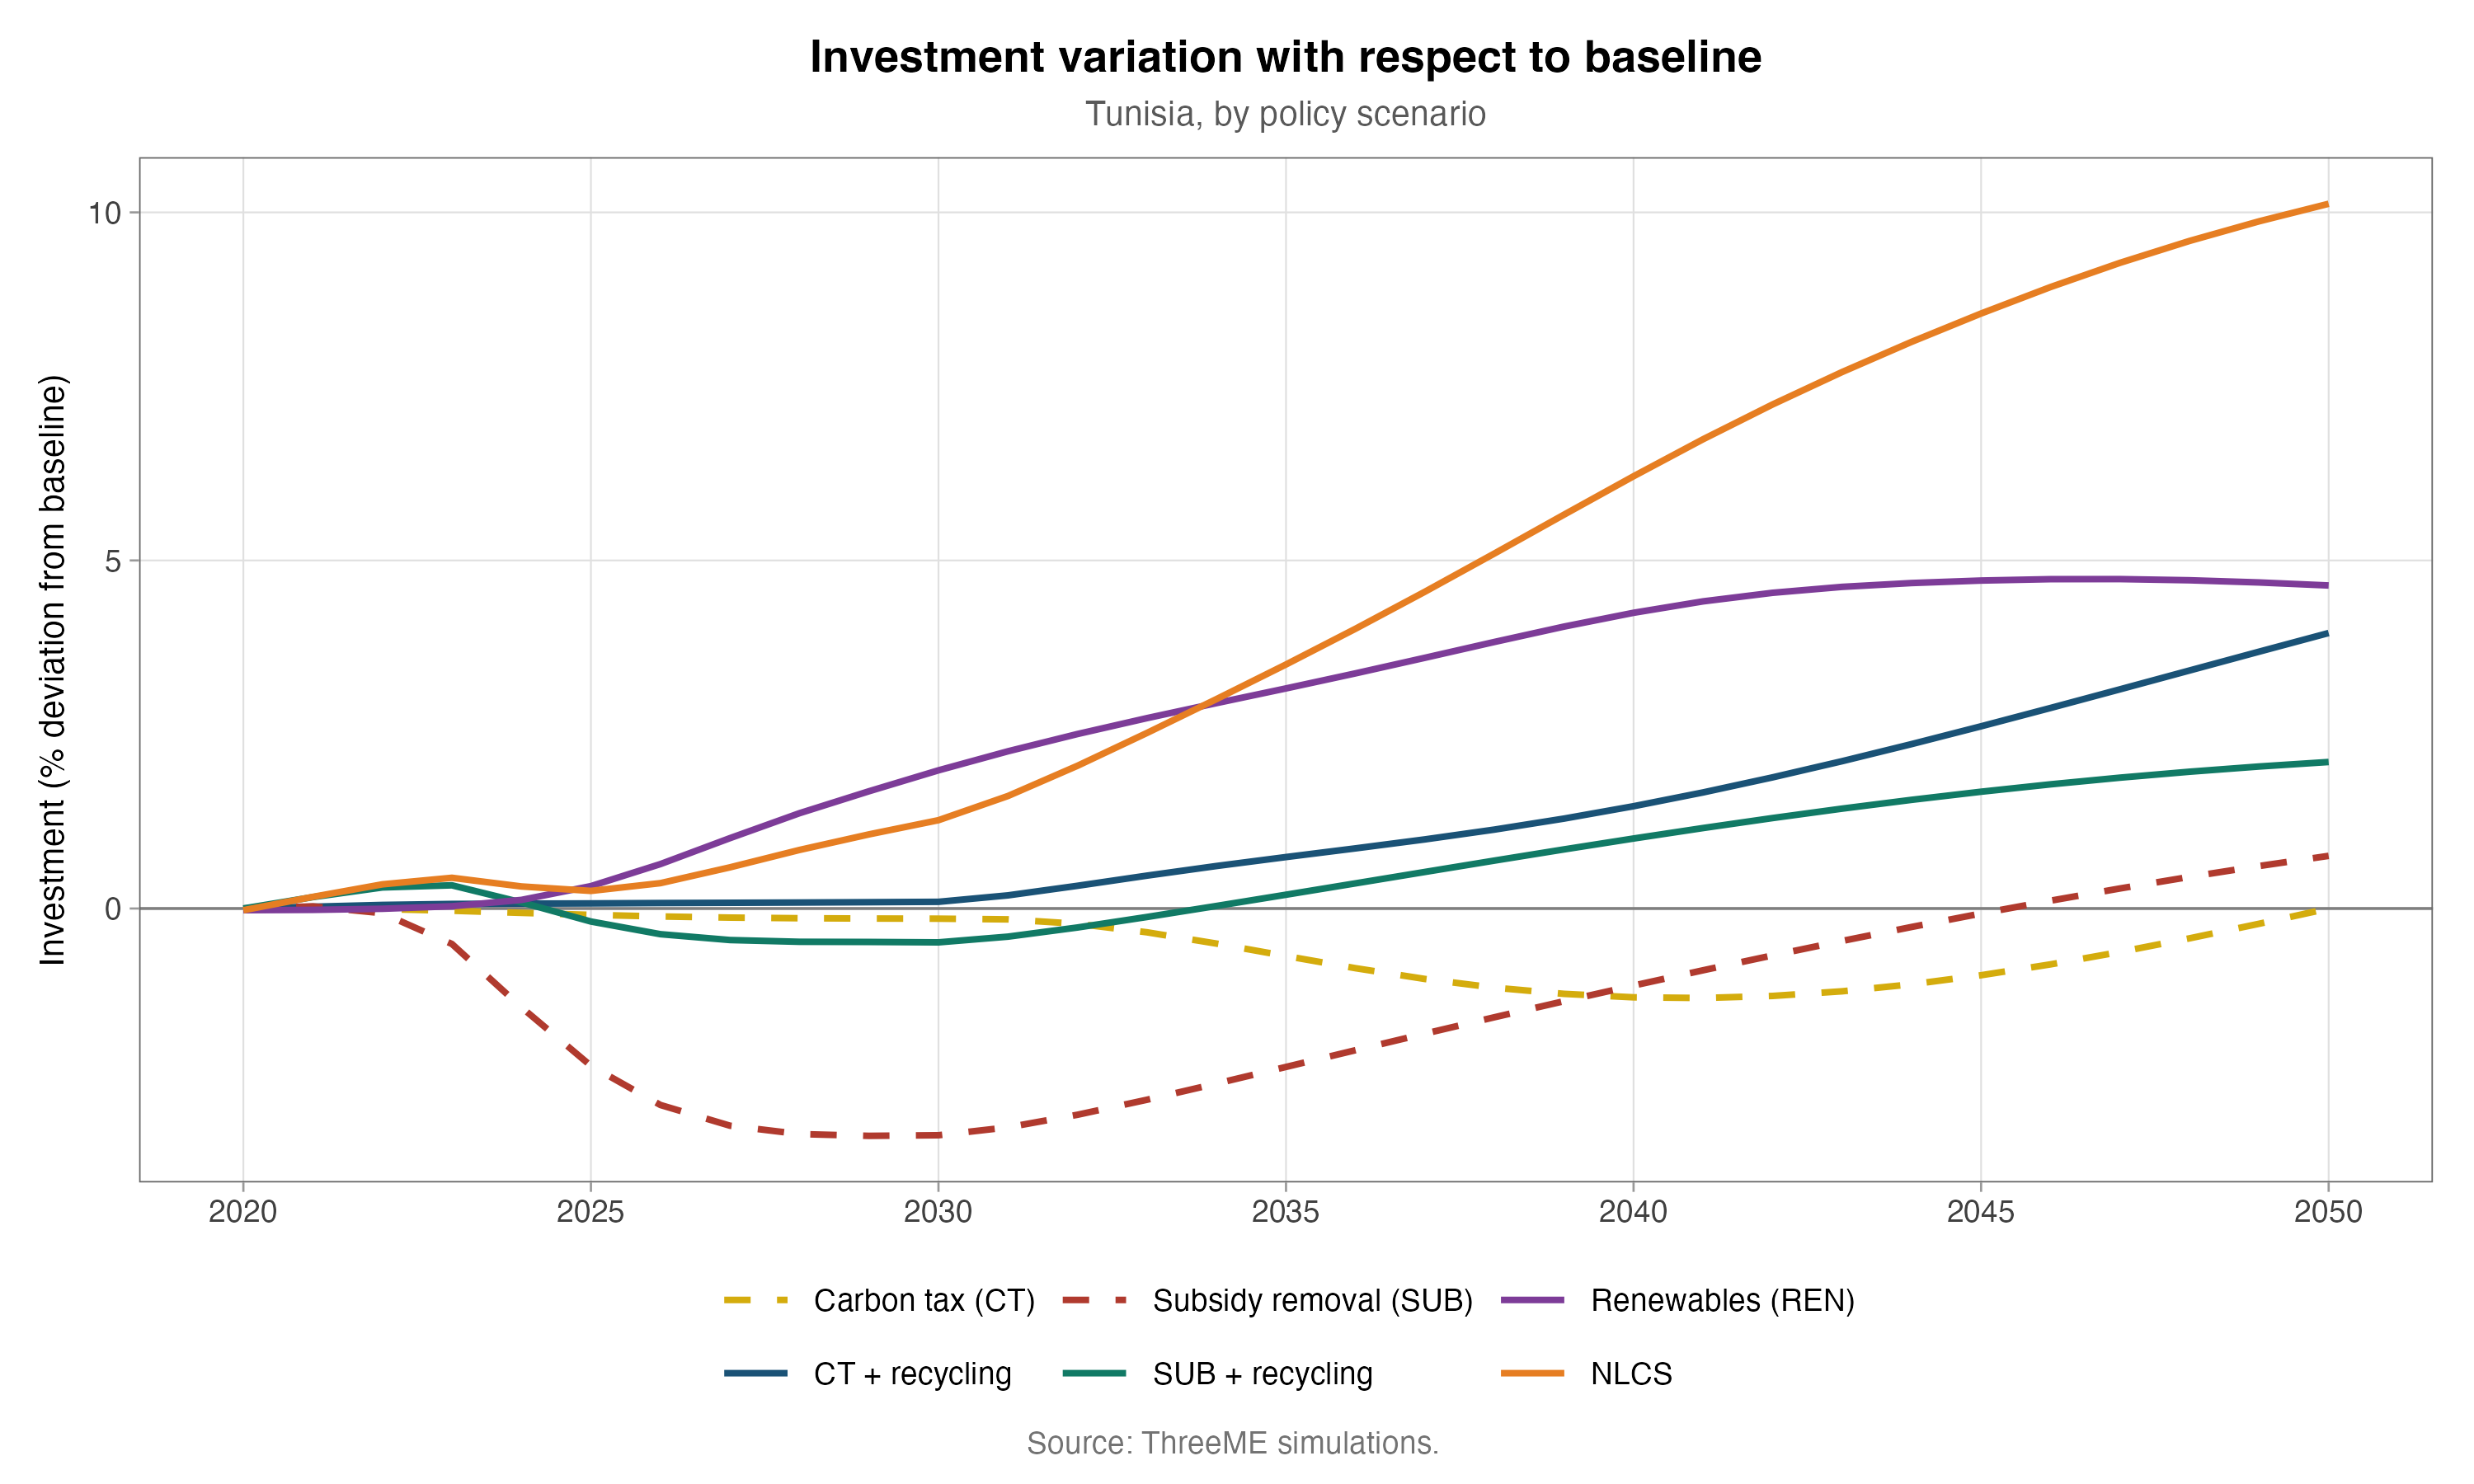
\includegraphics[width=0.95\textwidth]{fig09_investissement_scenarios.png}
    \caption{Investment variation by scenario with respect to baseline in Tunisia}
    \label{fig:invest_scenarios}
\end{figure}

In Tunisia, aggregate investment increases steadily in the scenarios based on renewable energy deployment, driven mainly by the construction of renewable electricity generation infrastructure and the modernisation of the grid (Figure~\ref{fig:invest_scenarios}). The most striking effects are observed in the full NLCS scenario: the introduction of progressive carbon taxation, combined with incentive price signals and the recycling of public revenues, significantly stimulates investment activity. In 2050, investment stands 12\% above its baseline level.

\begin{figure}[H]
    \centering
    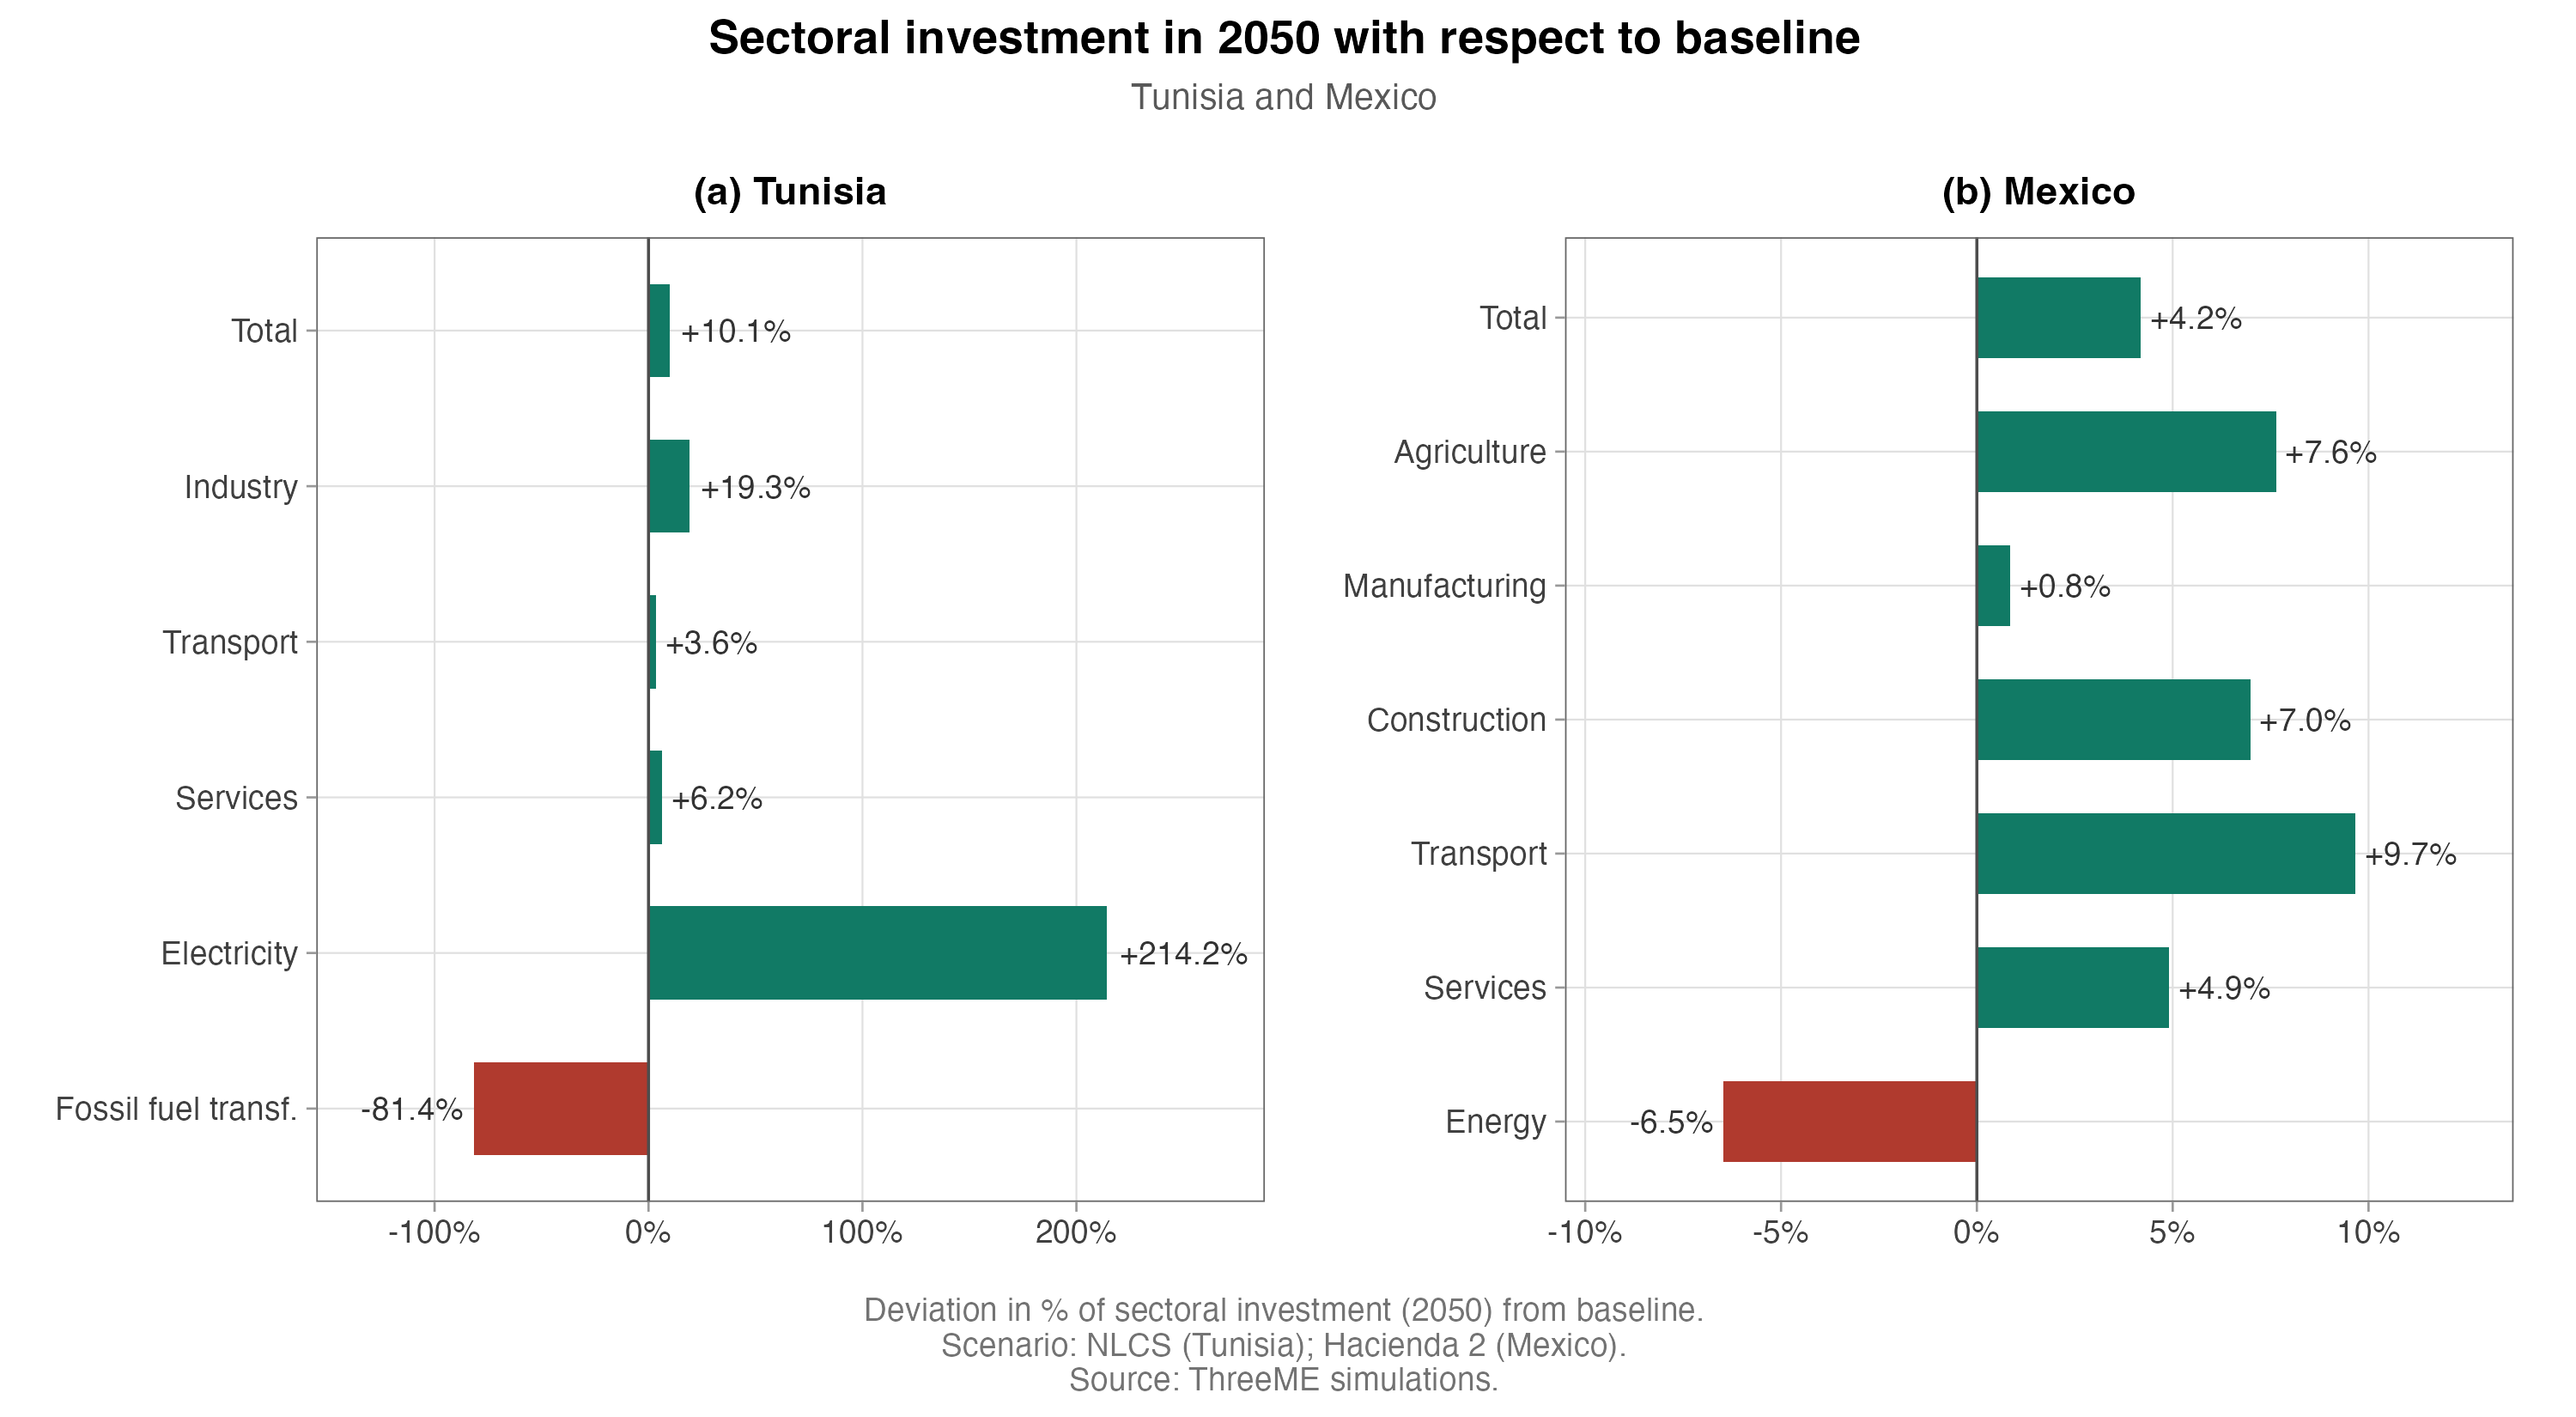
\includegraphics[width=0.95\textwidth]{fig10_investissement_sectoriel.png}
    \caption{Sectoral investment in 2050 with respect to baseline in Tunisia (NLCS) and Mexico}
    \label{fig:invest_sectoral}
\end{figure}

The sectoral analysis of investment (Figure~\ref{fig:invest_sectoral}) reveals contrasting dynamics between the two countries. The low-carbon strategy induces a significant increase in investment in certain sectors, notably industry and electricity. Given the very strong constraint imposed on the renewal of the electricity mix, investment in the electricity sector rises sharply. In Tunisia, investment in this sector increases by +66\% in 2030, +160\% in 2040 and +210\% in 2050 relative to the baseline. A substitution effect then occurs: investment in fossil fuels simultaneously falls markedly.

\subsection{Energy consumption and emissions by sector}
\label{subsec:energy_emissions}

The shocks induced by the removal of fossil fuel subsidies and the introduction of a carbon tax generate a decline in the energy consumption of households and productive sectors. For Tunisia, household energy consumption falls by 8\% from the first year relative to the baseline, and this gap keeps widening to reach 36\% by 2050.

\begin{figure}[H]
    \centering
    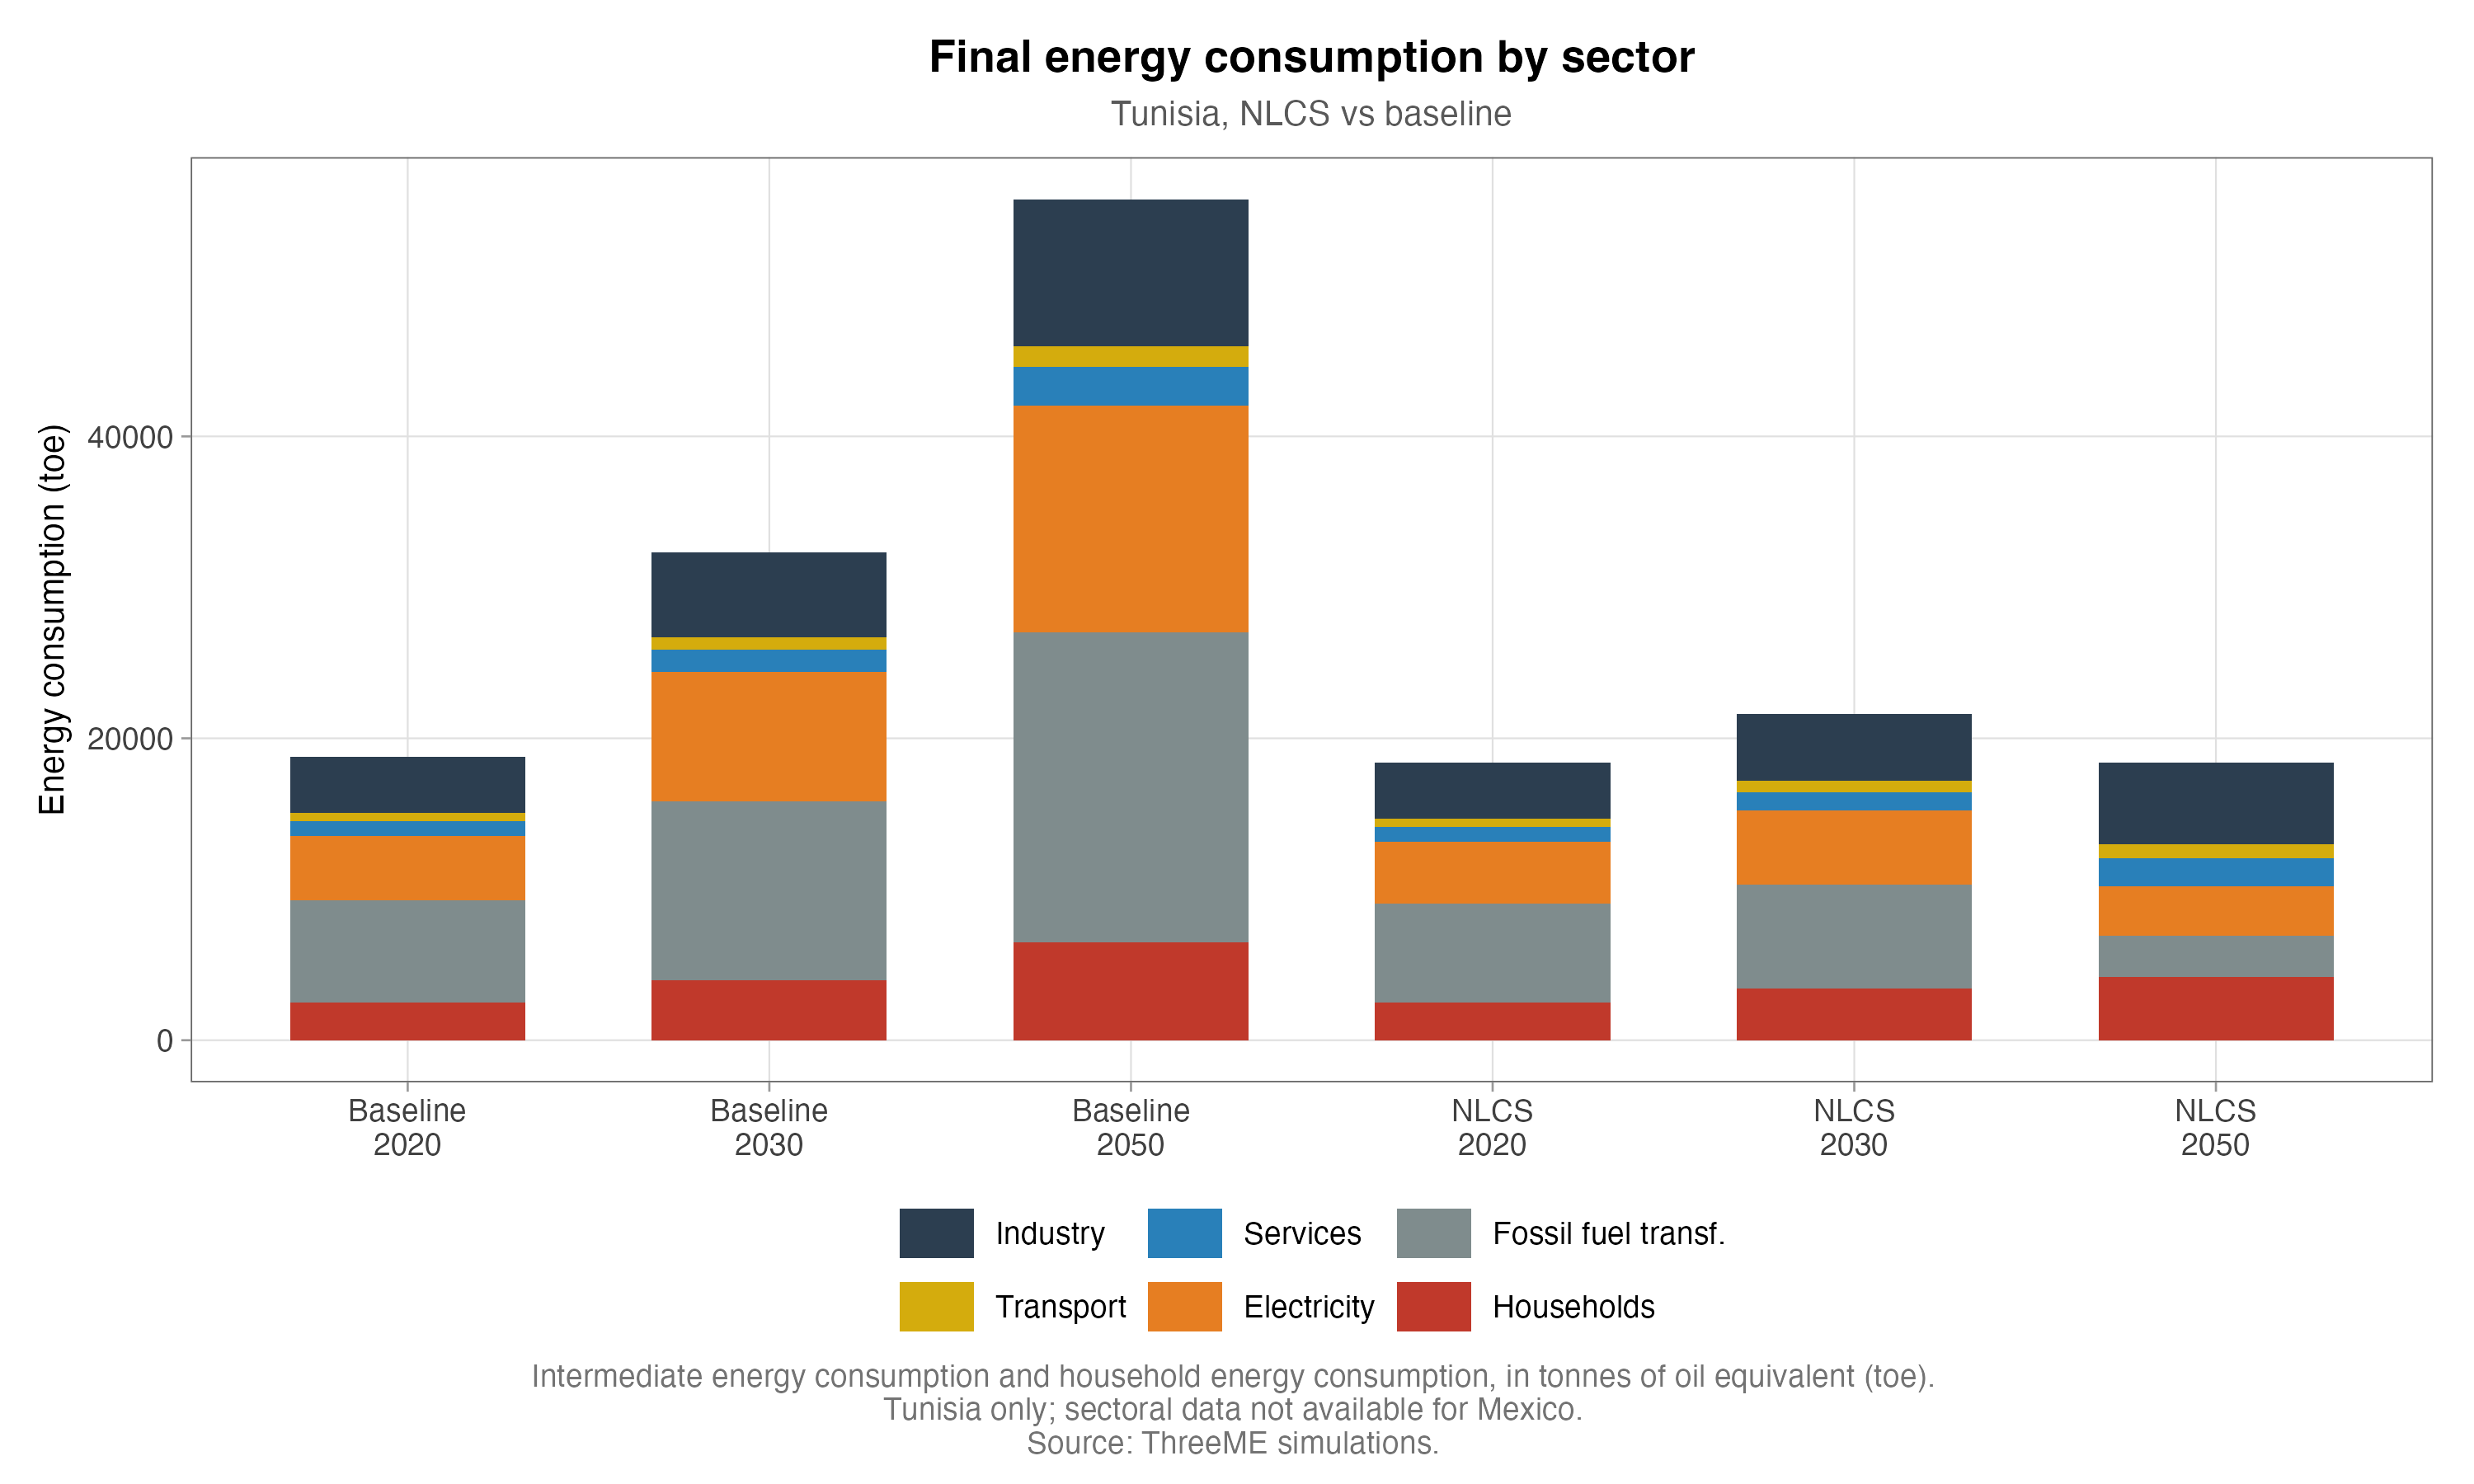
\includegraphics[width=0.95\textwidth]{fig11_energie_sectorielle.png}
    \caption{Final energy consumption by sector in Tunisia (NLCS vs.\ baseline)}
    \label{fig:energy_sector}
\end{figure}

Given the massive electrification of uses and the significant penetration of renewables in the electricity mix, this decline in household consumption is accompanied by an even larger decline in their CO$_2$ emissions (Figure~\ref{fig:co2_sector}). The CO$_2$ emissions of Tunisian households fall by 60\% in 2050, from 13\,MtCO$_2$ in the baseline to 5\,MtCO$_2$.

\begin{figure}[H]
    \centering
    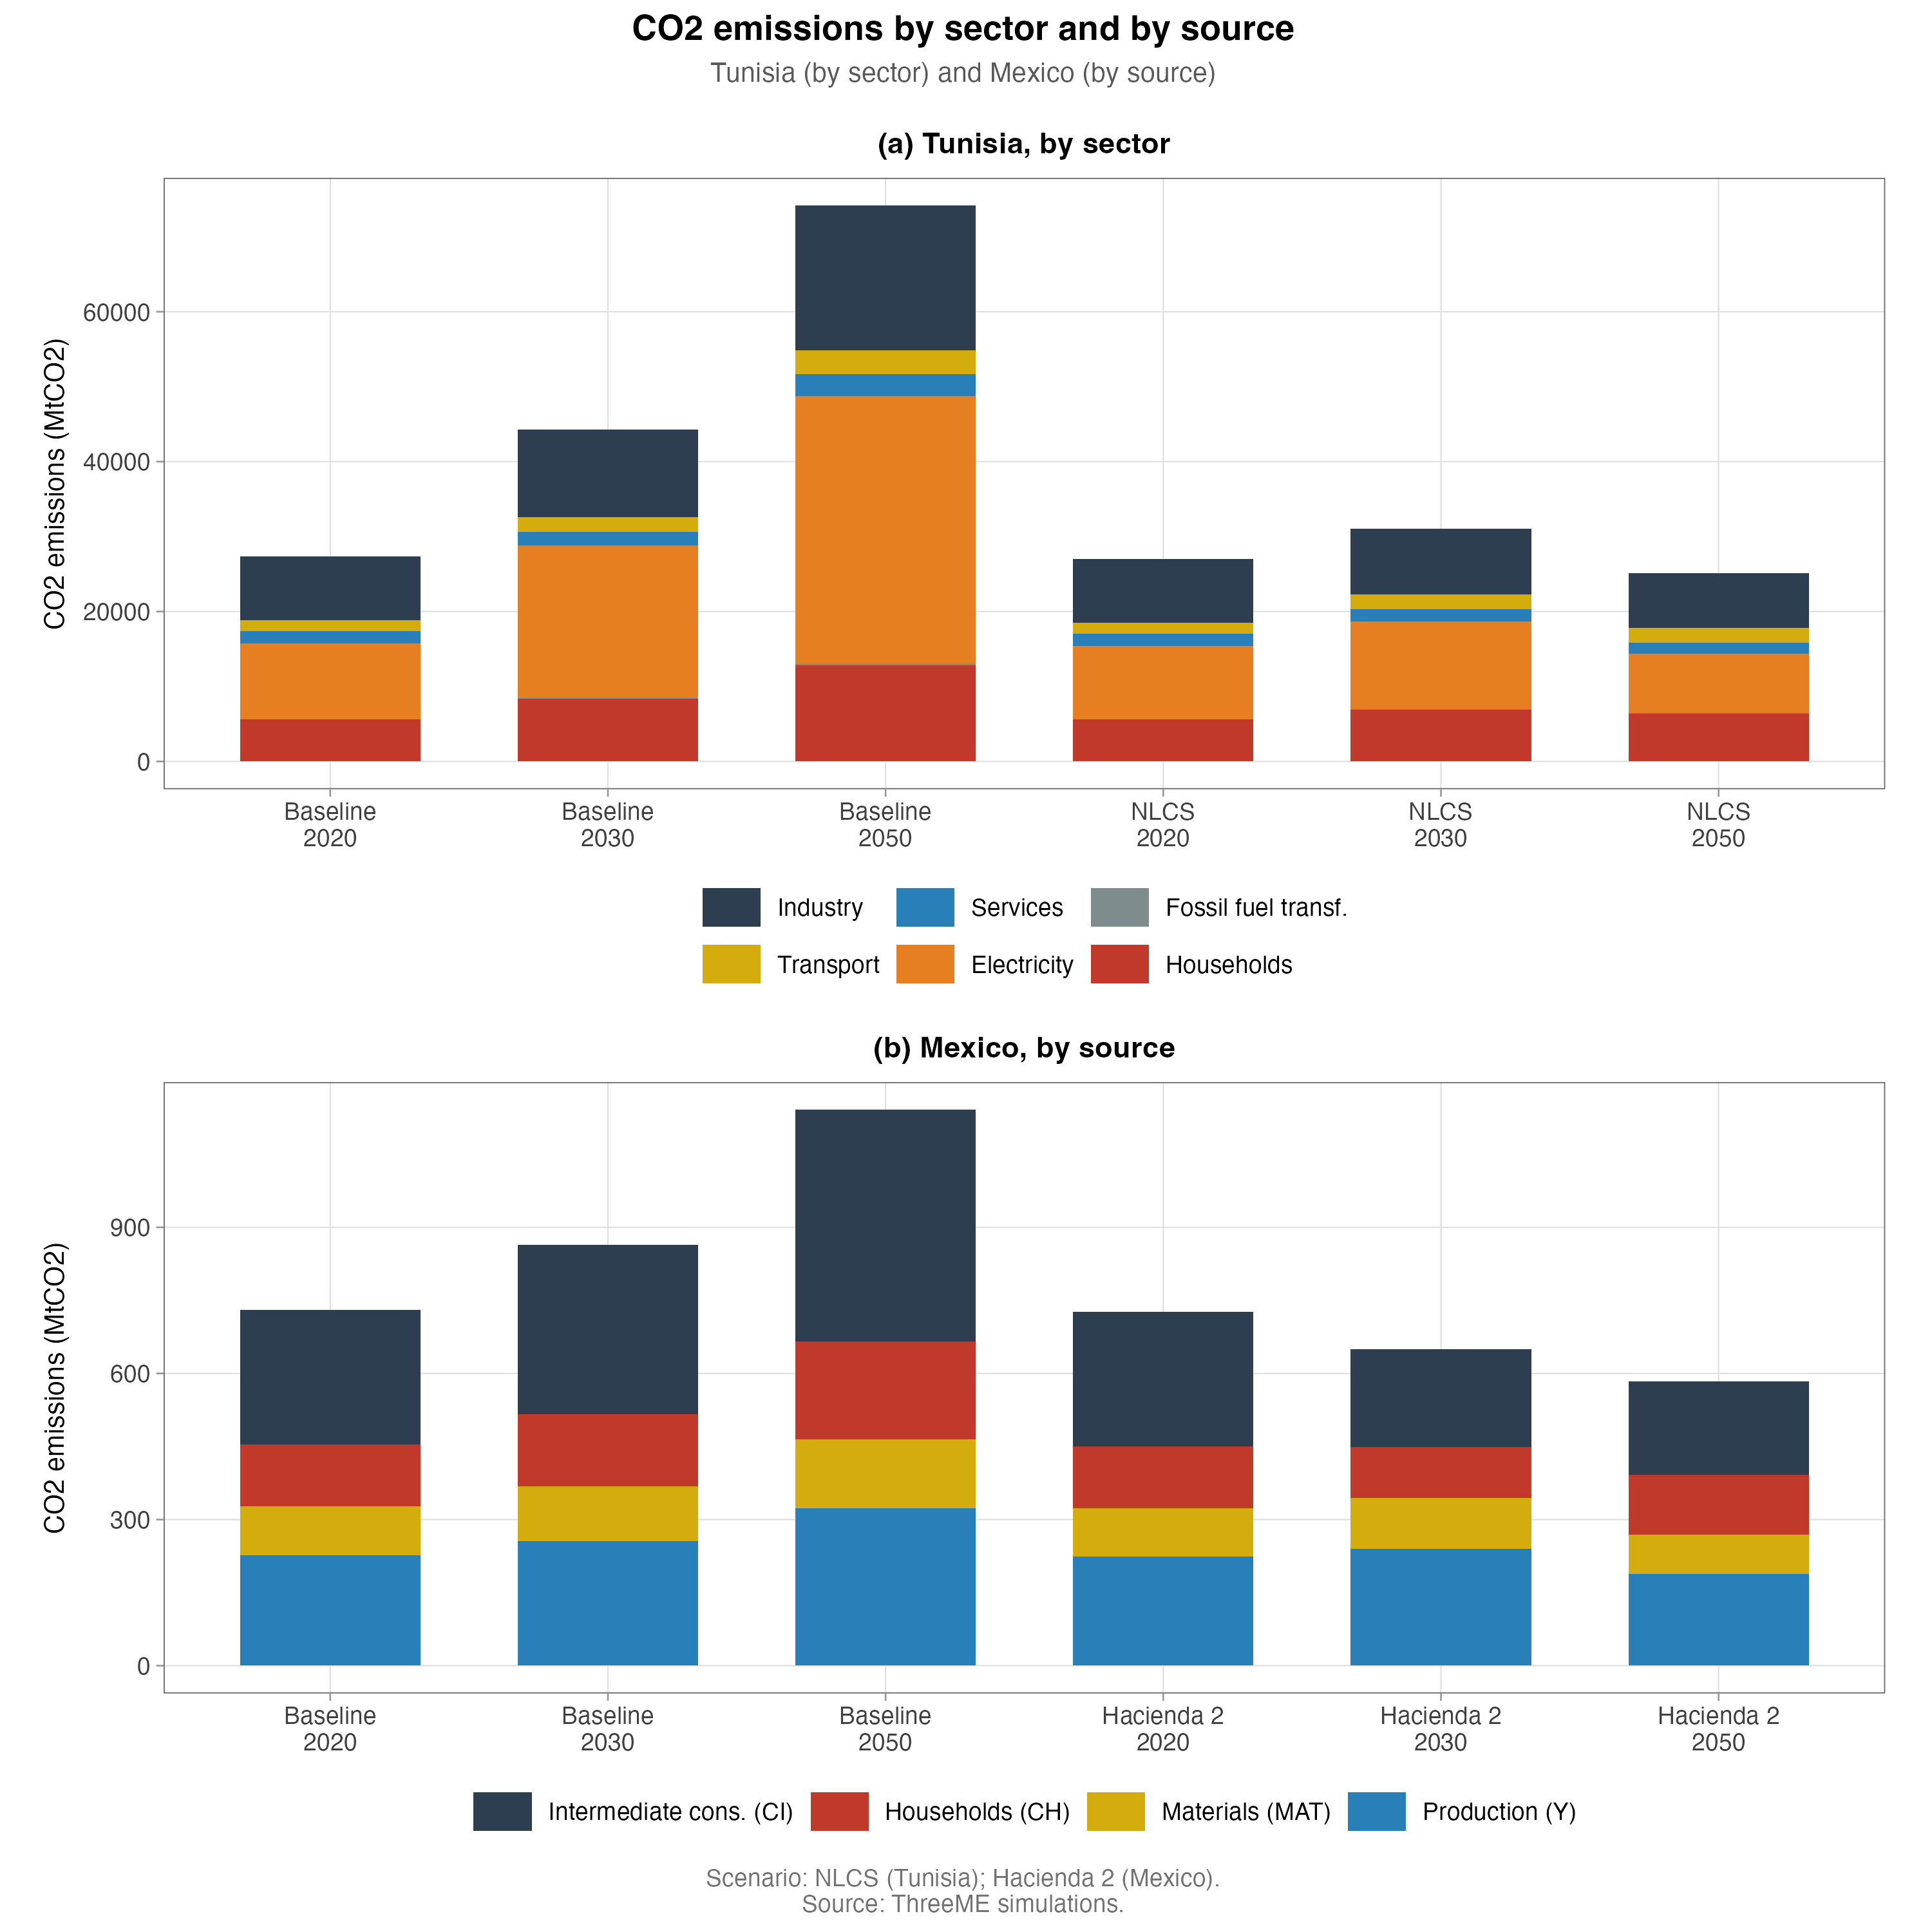
\includegraphics[width=0.95\textwidth]{fig12_co2_sectoriel.png}
    \caption{CO$_2$ emissions by sector in Tunisia (NLCS vs.\ baseline) and by source in Mexico}
    \label{fig:co2_sector}
\end{figure}

The same phenomena are observed in the productive sectors, but with a lower intensity at the start of the policy implementation. Conversely, the decline in energy consumption is more pronounced at the end of the period for these sectors: while households reduce their consumption by 36\% in 2050, the productive sectors reduce theirs by 69\%. Similarly for emissions, energy efficiency and the penetration of renewables in the electricity mix contribute to a significant reduction: $-57$\% in services, $-65$\% in industry and $-85$\% in electricity in 2050 relative to the baseline.

\subsection{Sectoral reallocation of value added}
\label{subsec:reallocation}

\begin{figure}[H]
    \centering
    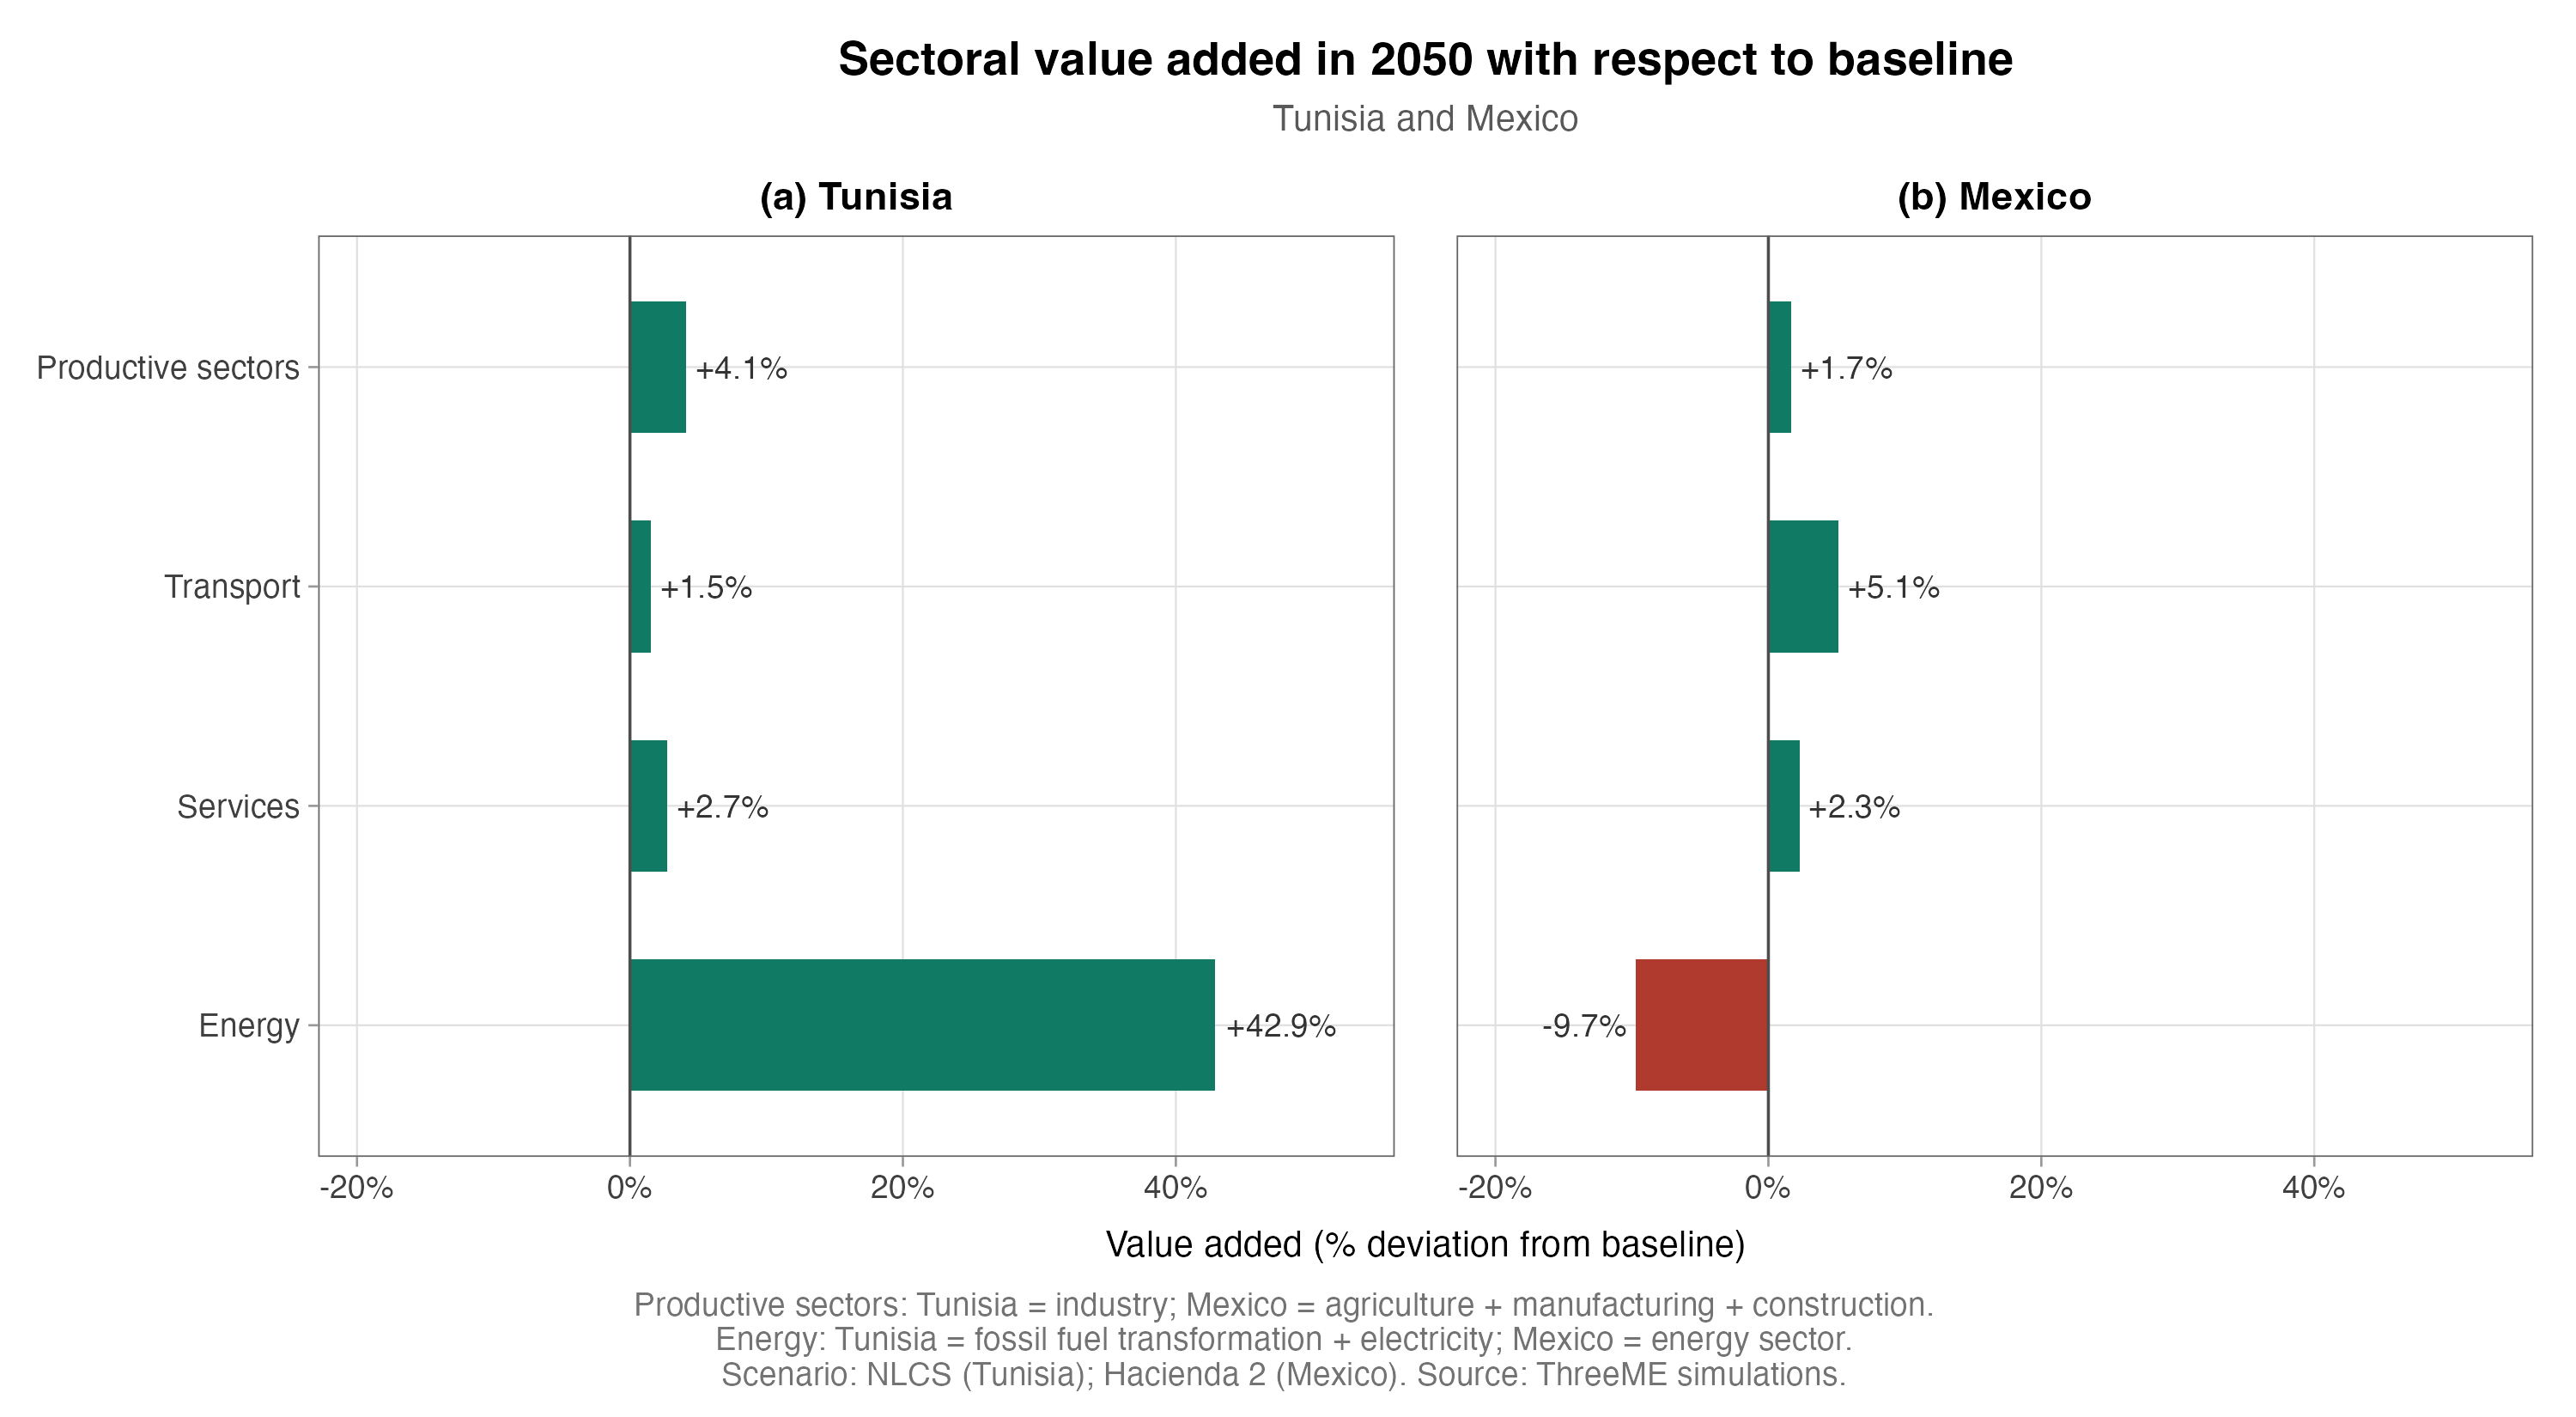
\includegraphics[width=0.95\textwidth]{fig06_va_sectorielle.png}
    \caption{Sectoral reallocation of value added in Tunisia and Mexico}
    \label{fig:sectoral_va}
\end{figure}

While the services, transport and industrial sectors remain relatively stable and display comparable evolutions in Tunisia and Mexico, the energy sector undergoes strong and opposite variations in the two countries (Figure~\ref{fig:sectoral_va}).

On one side, the energy sector contracts by 7\% relative to the baseline in Mexico. The carbon tax makes fossil hydrocarbon exports less competitive: this is the end of the fossil rent from which Mexico benefited. By contrast, the transition allows Tunisia to reduce its external dependence on imported hydrocarbons. The development of renewable energy drives strong growth in the energy sector through the relocation of production.

Another mechanism comes into play: the improvement in the price competitiveness of exporting sectors (manufacturing industry and services), financed by the reduction of production taxes thanks to carbon tax revenues.

\subsection{Labour market effects}
\label{subsec:employment}

One of the most striking lessons of the simulations concerns labour market effects, which materialise progressively over time depending on the intensity and combination of the policies implemented. In Tunisia, the integrated NLCS scenario leads to a net creation of 51,000 jobs by 2030, which steadily expands to reach 194,000 additional jobs in 2050. These results illustrate the capacity of the transition to mobilise new skills, stimulate private and public investment, and reorient the productive fabric towards more labour-intensive sectors.

\begin{figure}[H]
    \centering
    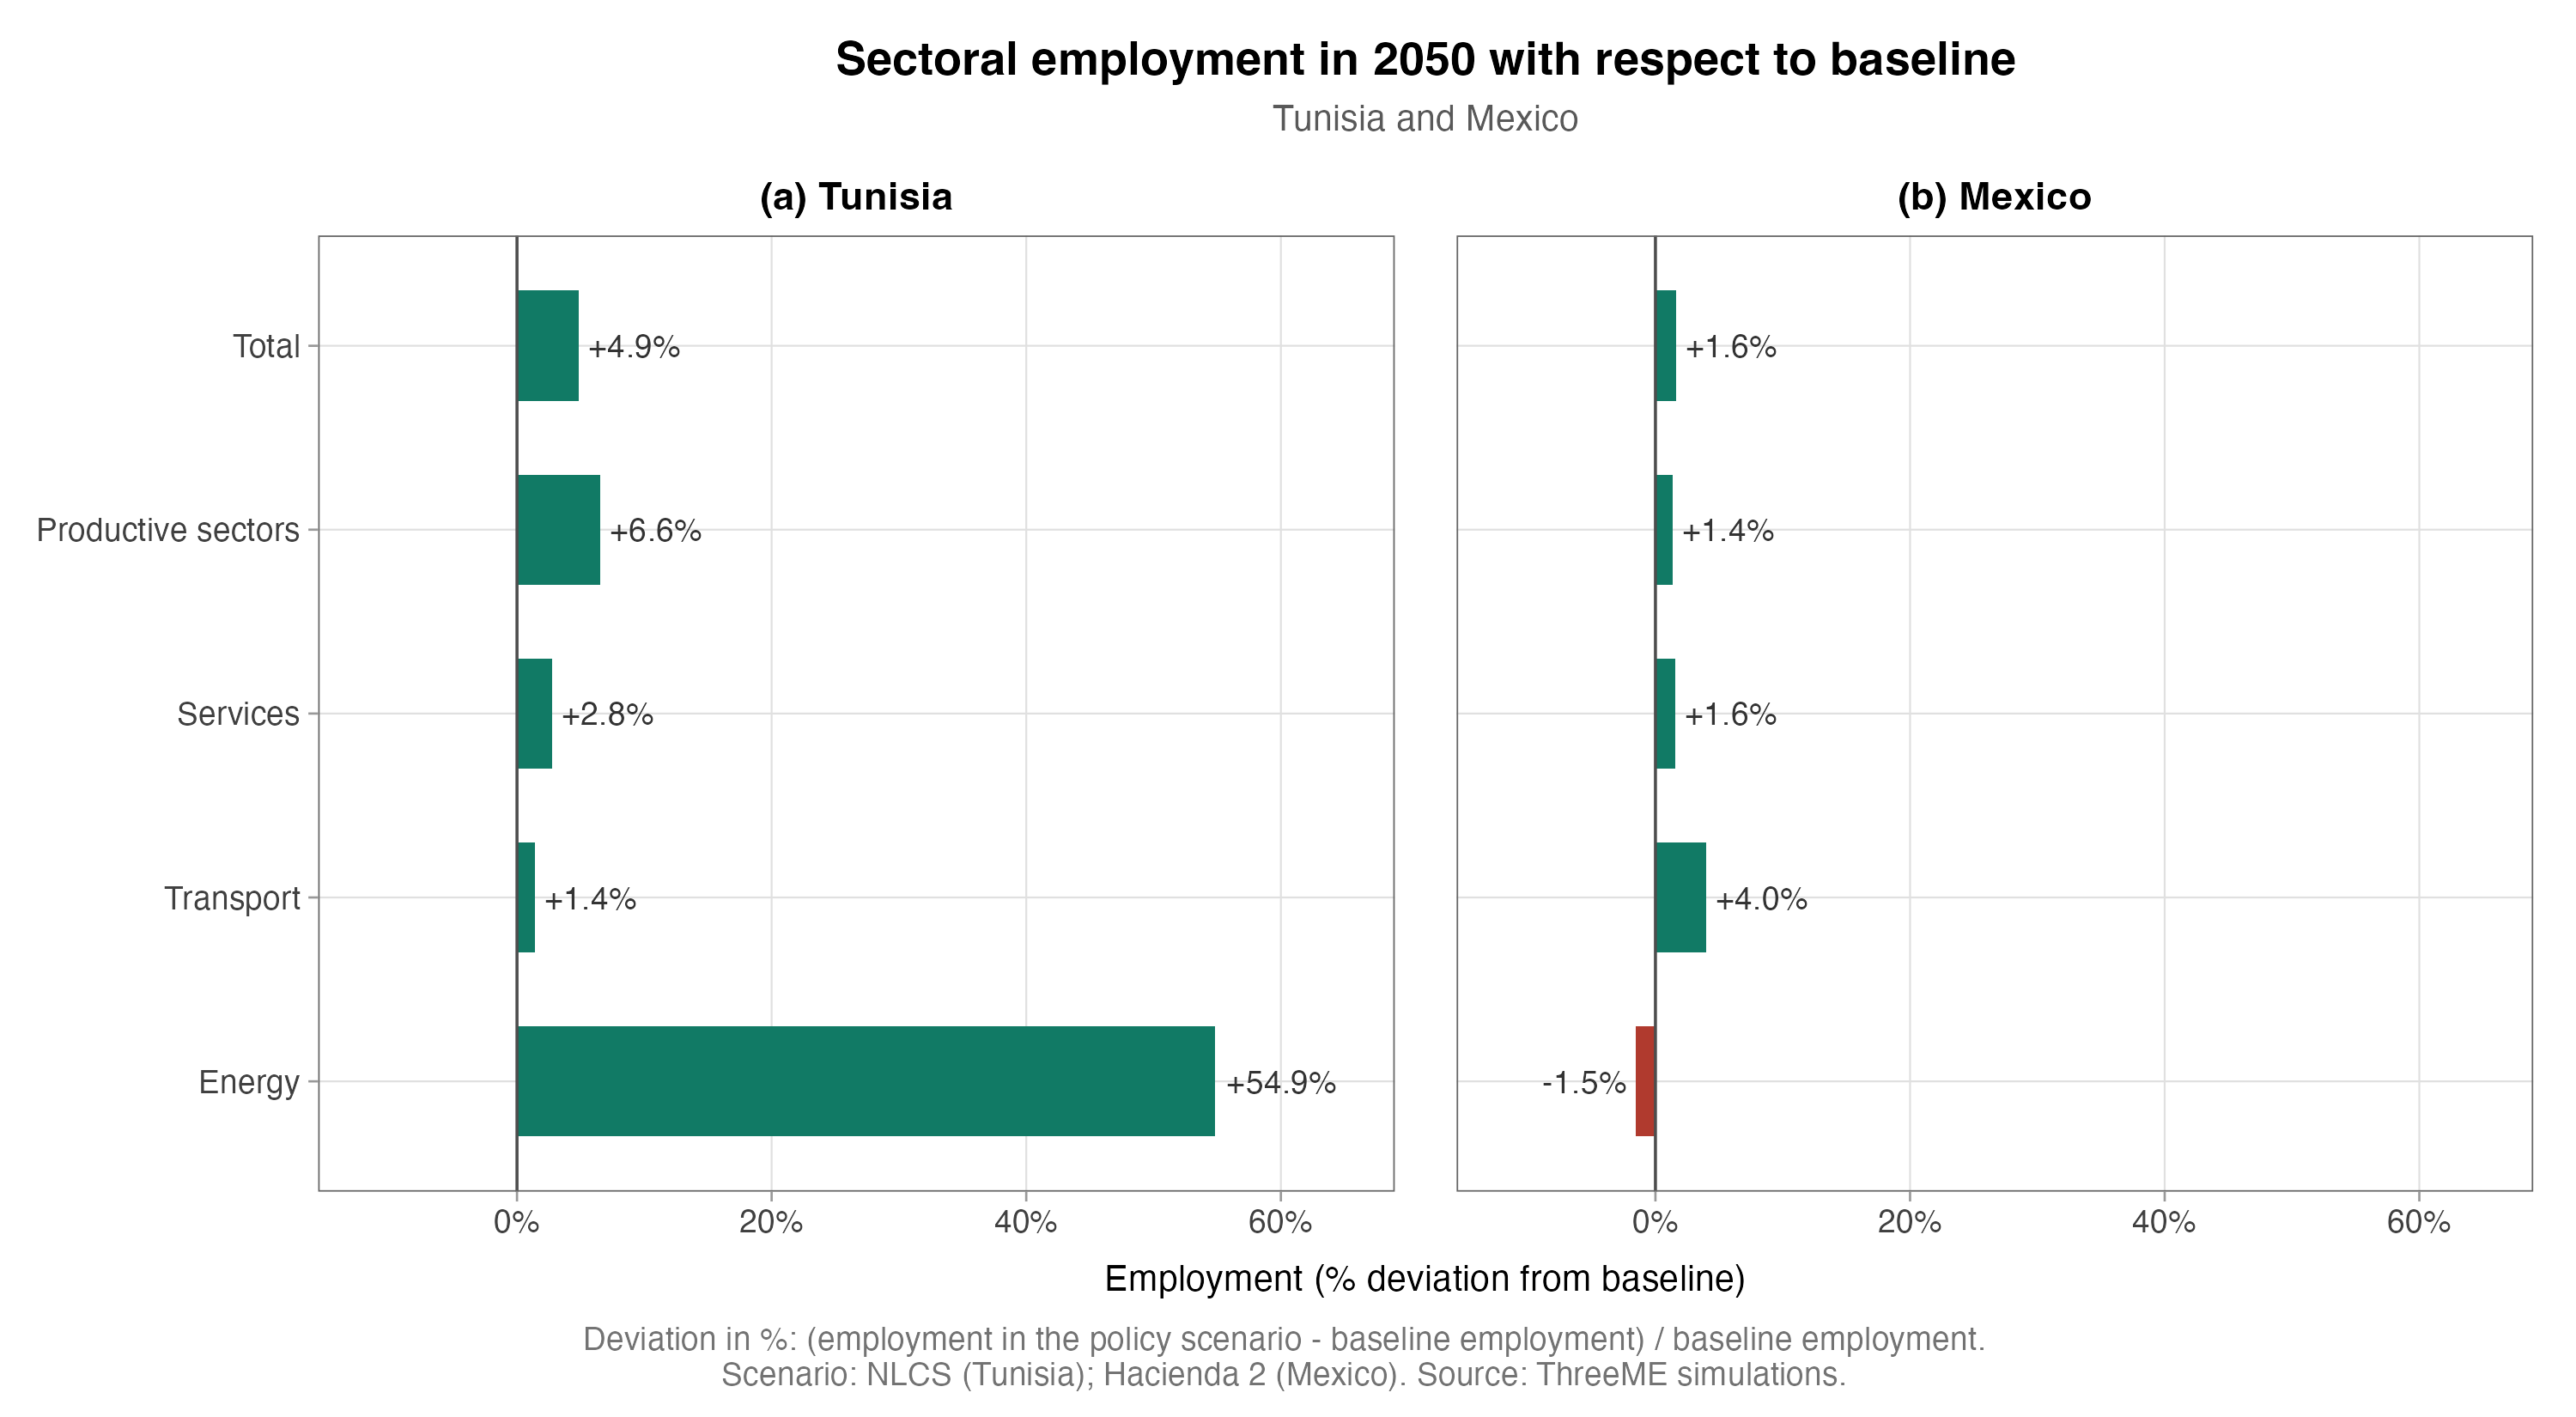
\includegraphics[width=0.95\textwidth]{fig07_emploi_sectoriel.png}
    \caption{Sectoral employment effects in Tunisia and Mexico in 2050}
    \label{fig:employment_sectors}
\end{figure}

For Mexico (Figure~\ref{fig:employment_sectors}), aggregate job creation exceeds one million jobs in 2050, but the sectoral analysis shows that manufacturing employment drops by nearly 200,000 jobs in 2050, highlighting the structural reallocation effects that create winners and losers. The challenge for Mexico remains the conversion from crude oil exports to the development of its other sectors.

\subsection{Trade balance and external position}
\label{subsec:trade_balance}

\begin{figure}[H]
    \centering
    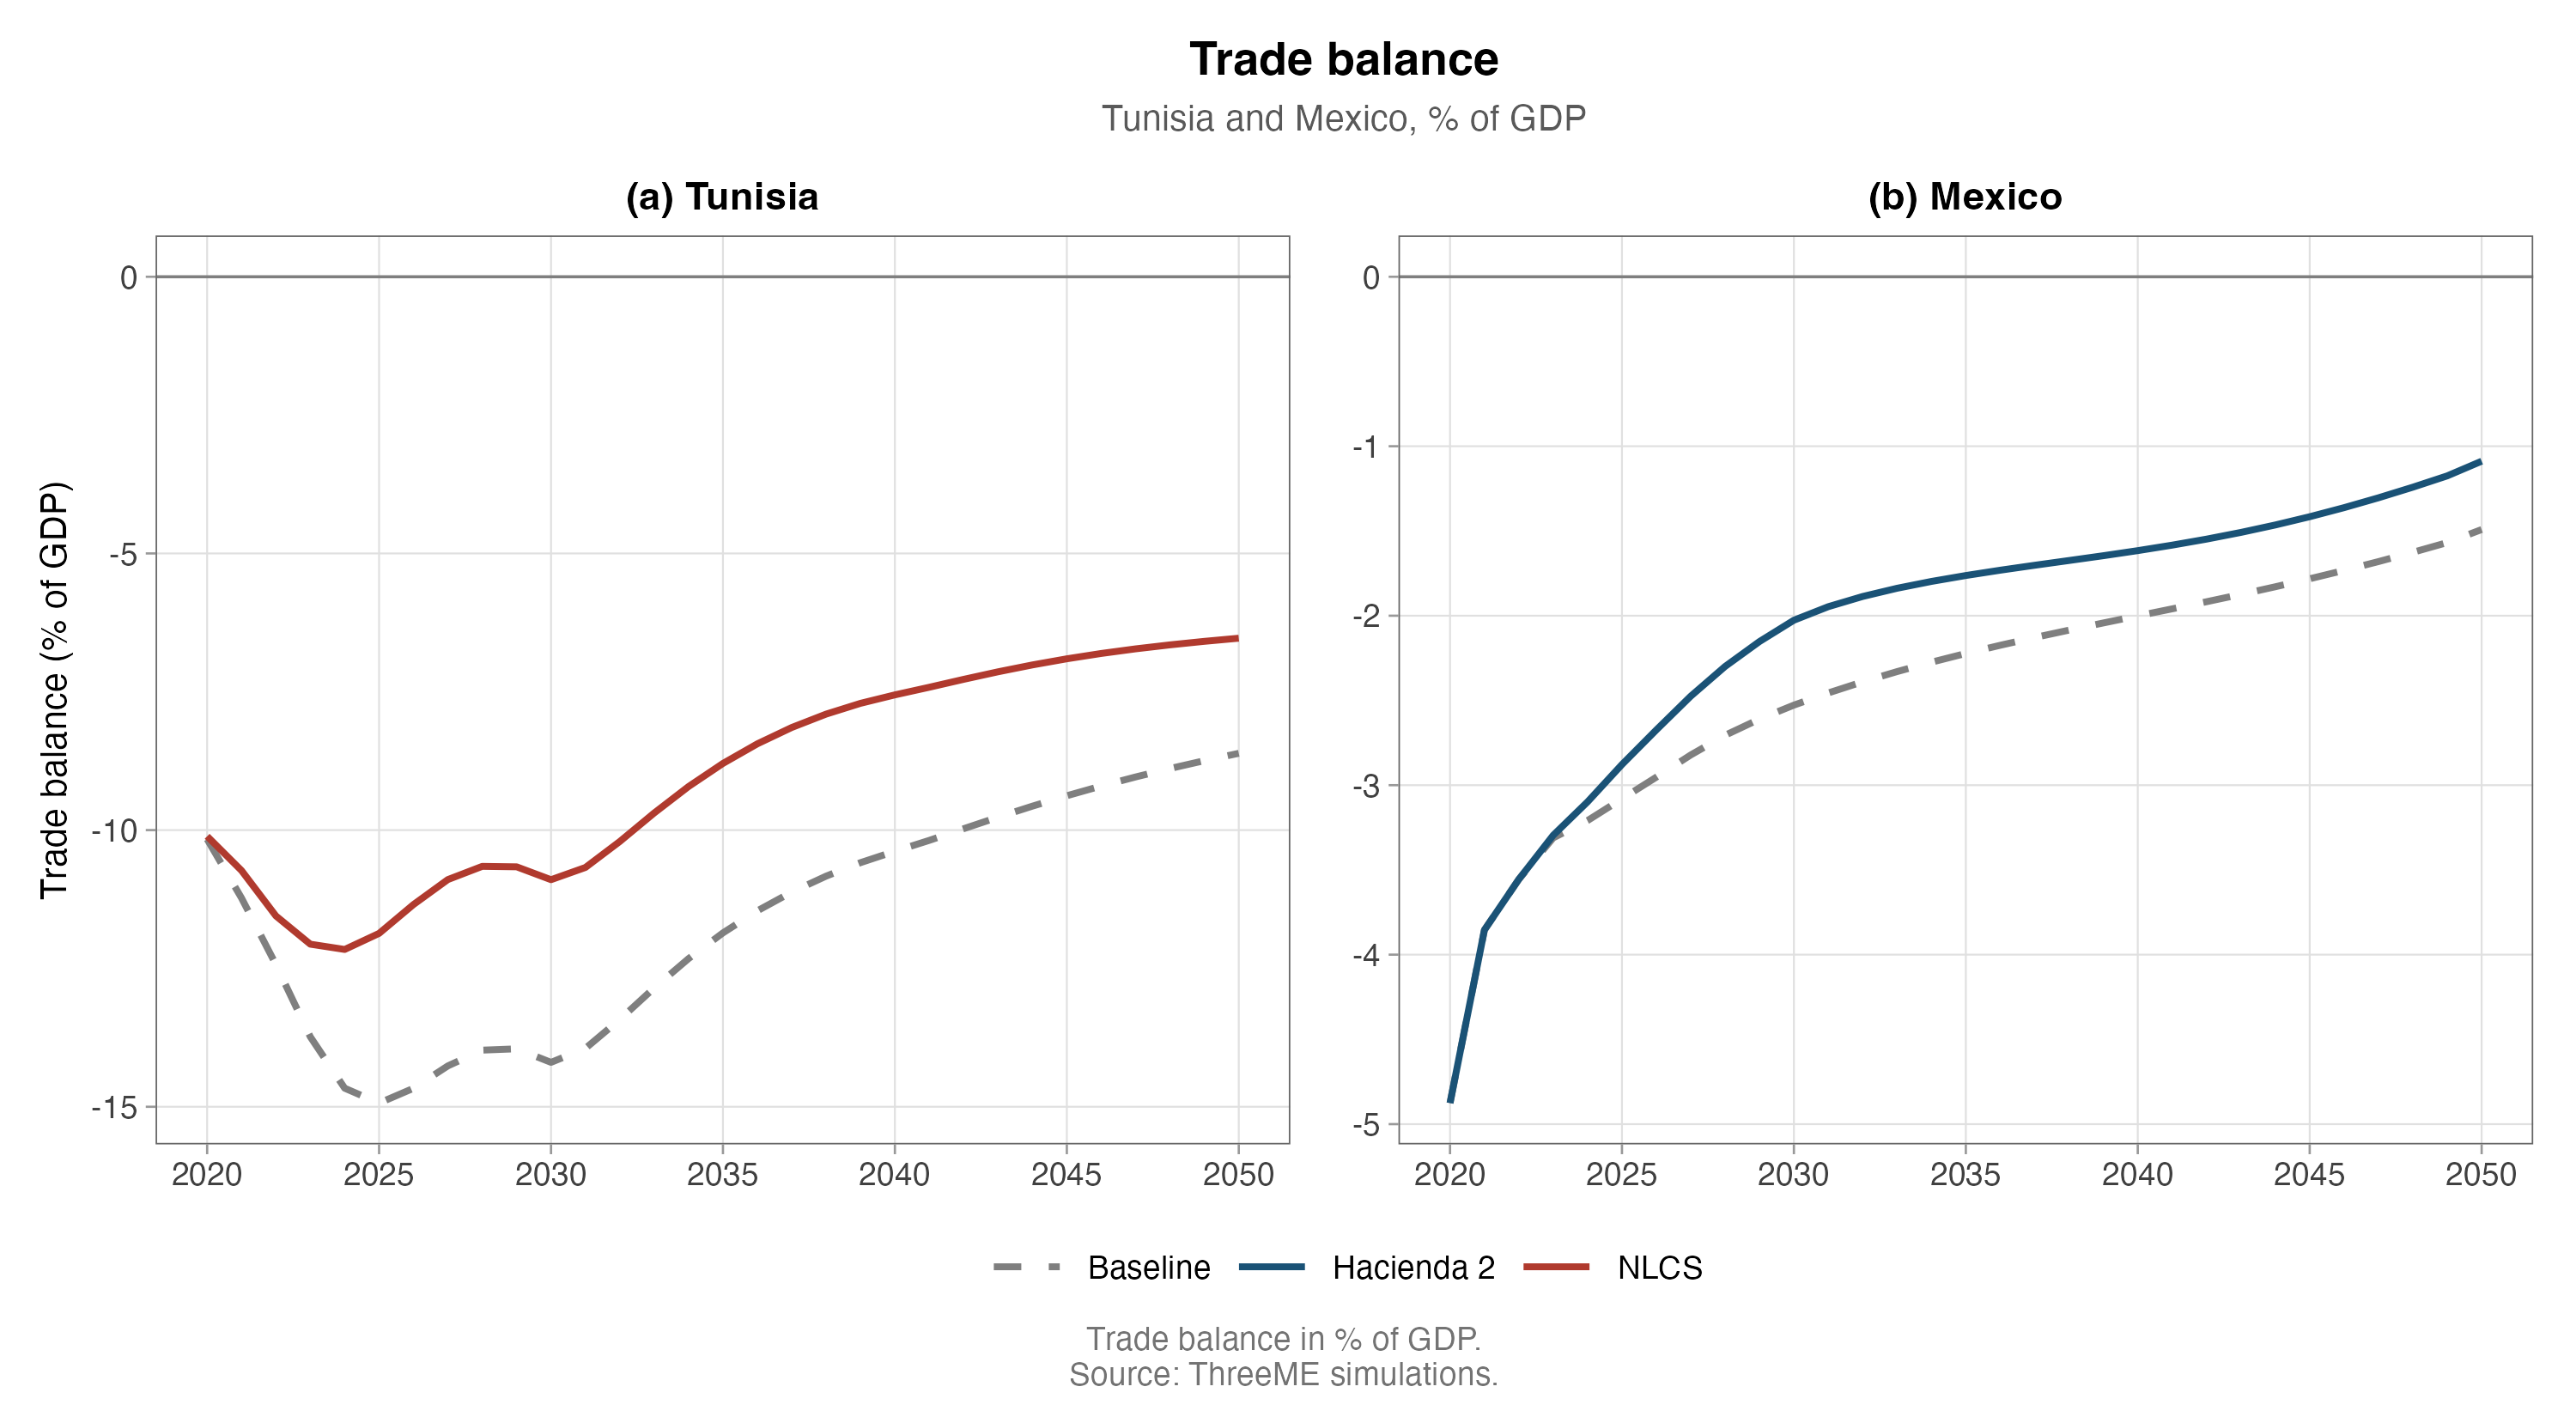
\includegraphics[width=0.95\textwidth]{fig13_balance_commerciale.png}
    \caption{Trade balance in Tunisia and Mexico (\% of GDP)}
    \label{fig:trade_balance}
\end{figure}

The trade balance is a revealing indicator of the asymmetry between the two countries (Figure~\ref{fig:trade_balance}). In Tunisia, the progressive reduction of fossil fuel imports mechanically improves the trade balance, strengthening the country's energy sovereignty. However, this improvement is partially offset by higher imports of capital goods required for the deployment of renewable infrastructure, particularly as long as local industrial capacities are not yet fully developed. The endogenous economic dynamics, supported by consumption and investment, also generate additional import demand.

In Mexico, the effect on the trade balance is more mixed. The fall in hydrocarbon exports directly weighs on the trade balance, while the development of renewable sectors only partially offsets this loss, as Mexico must also import technologies and capital goods for its transition.

% ========================================
% 5. DISCUSSION
% ========================================
\section{Discussion: how realistic is the simulated decoupling?}
\label{sec:discussion}

The results presented suggest that, for both Tunisia and Mexico, a decoupling occurs between GDP growth and emission growth. This observation nevertheless depends on modelling assumptions whose robustness deserves discussion.

\textbf{Capital-energy substitution elasticities} determine how firms replace fossil energy with productive capital in response to the price signal. The larger the elasticity, the more easily decoupling occurs, yet this parameter is empirically debated (Landa \& Reynès, 2025). \textbf{Renewable penetration} is a scenario parameter imposed exogenously (80\% for Tunisia and 50\% for Mexico). If deployment proves more difficult or costly than expected, a different decoupling would be observed. \textbf{Fiscal recycling} mechanically increases the numerator of the GDP-growth-to-emission-growth ratio; the actual decarbonisation of the productive system stems from a mechanism separate from the macroeconomic effect.

Moreover, these assumptions confront contradictory empirical evidence. Haberl et al. (2020) show that examples of long-run absolute decoupling remain rare. Even where some post-industrial economies have achieved such decoupling, it would not be fast enough to meet the Paris Agreement objectives (Hickel \& Kallis, 2020). The decoupling mechanism may also be overestimated due to the territorial scope of emissions accounting, which does not capture carbon leakage: carbon-intensive goods could be imported by Tunisia rather than produced domestically.

Some transition-related costs are not modelled in ThreeME: the informal share of the Tunisian economy, the close link between PEMEX and public finances in Mexico, and the training required for labour market restructuring. In addition, general equilibrium models such as ThreeME capture only part of rebound effects, essentially the direct household rebound through prices and real income, leaving aside many economy-wide macroeconomic mechanisms (Brockway et al., 2021).

Finally, the comparability of results between the two countries is limited by the fact that the two versions of the model were developed and calibrated independently. Differences in sectoral structure, number of sectors, calibration of behavioural parameters and baseline assumptions call for a comparative reading centred on qualitative mechanisms rather than absolute magnitudes.

The results demonstrating decoupling are therefore strongly conditional. The lessons to be drawn are not the quantitative precision of the simulations, but the illustration of the mechanisms at work in the asymmetries between importers and exporters during the transition.

% ========================================
% 6. CONCLUSION
% ========================================
\section{Conclusion}
\label{sec:conclusion}

This paper provides an assessment of the macroeconomic effects of implementing national low-carbon strategies in two developing economies with contrasting energy profiles: Tunisia, a net importer of hydrocarbons, and Mexico, a net exporter. Using the neo-Keynesian computable general equilibrium model ThreeME, we simulate ambitious transition scenarios up to 2050.

In addition to the environmental dividend obtained by construction, our simulations show that transition policies can deliver an economic dividend: higher investment, and job creation in green industries that clearly exceeds job destruction in fossil-fuel-intensive sectors. Despite higher energy prices, demand increases and GDP exceeds its baseline level. For Tunisia, the transition yields a GDP gain of about +5\% and a significant employment gain in 2050. For Mexico, the gain is positive but more moderate, reflecting the cost of restructuring the extractive sector.

The comparison between Tunisia and Mexico highlights the asymmetric nature of the transition shock. For a net energy importer, the reduction of the external energy bill and the rise of domestic investment turn the transition into a lever for economic stimulus and trade balance improvement. Conversely, for a hydrocarbon exporter, the transition implies a more costly process of sectoral reallocation, marked by the decline of a historically central sector and by greater needs for productive and social support. The results also underline the importance of the time dimension: the effects are first dominated by investment, before structural reallocations become predominant as the carbon price rises.

Full recycling of fiscal revenues, through transfers to households and support for firms' productive investment, appears to be a necessary condition for obtaining the double dividend. Without recycling, the Tunisian scenarios show a GDP contraction relative to the baseline, confirming that the way revenues are redistributed matters as much as the level of the tax itself.

As discussed in Section~\ref{sec:discussion}, the decoupling observed in the simulations rests on a set of structuring assumptions whose realisation is not guaranteed. The model captures neither carbon leakage, nor household heterogeneity, nor retraining costs, which calls for caution in interpreting the quantitative results.

These limitations do not detract from the qualitative significance of the main lessons. Beyond the Tunisian and Mexican cases, this study suggests that the low-carbon transition in developing countries should be approached as a long-term economic transformation strategy. It is not merely a climate constraint, but also a potential lever for reorienting the growth model, provided it is accompanied by coherent fiscal, industrial and social policies. Future work could deepen the analysis by integrating a finer disaggregation of households, an explicit representation of training and retraining policies, and a modelling of multilateral trade interactions allowing the question of carbon leakage to be addressed.

% ========================================
% DATA AVAILABILITY
% ========================================
\section*{Data availability}

The ThreeME simulation outputs for Tunisia and Mexico, together with the code used to process the data and generate all figures, will be deposited in a public repository and cited in the article upon acceptance, in line with the journal's research data and replication requirements. During the review process, the data and code are available from the authors upon reasonable request.

% ========================================
% REFERENCES
% ========================================
\newpage
\section*{References}

\begin{itemize}[label={}, leftmargin=2em, itemindent=-2em, itemsep=2pt]

\item ANME (2020). Plan Solaire Tunisien : études sur le potentiel des énergies renouvelables et de l'efficacité énergétique. Agence Nationale pour la Maîtrise de l'Énergie.

\item Aubert, D., \& Chiroleu-Assouline, M. (2019). Environmental tax reform and income distribution with imperfect heterogeneous labour markets. \textit{European Economic Review}, 116, 60--82.

\item Babonneau, F., Badran, A., Haurie, A., Schenckery, M., \& Vielle, M. (2023). GCC countries strategic options in a global transition to zero-net emissions. \textit{Environmental Modeling \& Assessment}, 28, 709--733.

\item Belhadj, A., Dakhlaoui, A., \& Gouider, R. (2022). Assessing macroeconomic, distributive, and environmental impacts of energy subsidy removal in Tunisia with input-output modeling. In \textit{Key Challenges and Policy Reforms in the MENA Region}, Springer, pp.~65--84.

\item Bento, A.~M., \& Jacobsen, M.~R. (2007). Ricardian rents, environmental policy and the `double-dividend' hypothesis. \textit{Journal of Environmental Economics and Management}, 53(1), 17--31.

\item Böhringer, C., Garcia-Muros, X., \& Gonzalez-Eguino, M. (2019). Greener and fairer: a progressive environmental tax reform for Spain. \textit{Economics of Energy \& Environmental Policy}, 8(2).

\item Böhringer, C., Rutherford, T.~F., \& Schneider, J. (2021). The incidence of CO$_2$ emissions pricing under alternative international market responses. \textit{Energy Economics}, 101, 105404.

\item Brockway, P.~E., Sorrell, S., Semieniuk, G., Heun, M.~K., \& Court, V. (2021). Energy efficiency and economy-wide rebound effects: A review of the evidence and its implications. \textit{Renewable and Sustainable Energy Reviews}, 141, 110781.

\item Bulavskaya, T., \& Reynès, F. (2018). Job creation and economic impact of renewable energy in the Netherlands. \textit{Renewable Energy}, 119, 528--538.

\item Callonnec, G., Landa, G., Malliet, P., Reynès, F., \& Tamsamani, Y. (2013). A full description of the ThreeME model. \textit{Document de travail OFCE}.

\item Callonnec, G., Landa, G., Malliet, P., Saussay, A., \& Reynès, F. (2016). Les propriétés dynamiques et de long terme du modèle ThreeME : un cahier de variantes. \textit{Revue de l'OFCE}, 149.

\item Callonnec, G., Gouëdard, H., Hamdi-Cherif, M., Landa, G., Malliet, P., Reynès, F., \& Saussay, A. (2025). Macroeconomic effects of achieving carbon neutrality in France. \textit{Energy and Climate Change}, 6, 100131.

\item Dridi, M. (2024). Tunisia: economic challenges and reform prospects. Working paper.

\item Elbargathi, K., \& Al-Assaf, G. (2019). The impact of political instability on the economic growth: an empirical analysis for the case of selected Arab countries. \textit{International Journal of Business and Economics Research}, 8(6), 353--360.

\item Fragkos, P., Fragkiadakis, K., \& Paroussos, L. (2021). Reducing the decarbonisation cost burden for EU energy-intensive industries. \textit{Energies}, 14(1), 236.

\item Goulder, L.~H. (2013). Climate change policy's interactions with the tax system. \textit{Energy Economics}, 40(Suppl. 1), S3--S11.

\item Haberl, H., et al. (2020). A systematic review of the evidence on decoupling of GDP, resource use and GHG emissions. \textit{Environmental Research Letters}, 15(6), 065003.

\item Hamdi-Cherif, M., Reynès, F., Landa, G., \& Wang, J. (2025). Effets macroéconomiques et environnementaux de la SNBC en Tunisie -- Une analyse à court et long terme. \textit{Revue de l'OFCE}.

\item Hickel, J., \& Kallis, G. (2020). Is green growth possible? \textit{New Political Economy}, 25(4), 469--486.

\item IEA (2021). Net Zero by 2050: A Roadmap for the Global Energy Sector. International Energy Agency.

\item IPCC (2018). Global Warming of 1.5\,$^{\circ}$C. Summary for Policymakers. IPCC, Geneva, Switzerland.

\item IPCC (2022). Climate Change 2022: Mitigation of Climate Change. Sixth Assessment Report.

\item Jacques, P., Augier, S., Barbosa, S., Yilmaz, S.~D., Jeanmart, H., \& Godin, A. (2025). Coupling a stock-flow consistent macroeconomic model with an energy system optimisation model to study the impacts of the energy transition in Colombia. \textit{SSRN Working Paper}, No.~5650377.

\item Jebali, E., et al. (2017). Energy consumption and economic growth in Tunisia. \textit{Journal of Policy Modeling}.

\item Kahn, J.~R., \& Farmer, A. (1999). The double dividend, second-best worlds, and real-world environmental policy. \textit{Ecological Economics}, 30, 433--439.

\item Karanfil, F., \& Omgba, L.~D. (2023). The energy transition and export diversification in oil-dependent countries: the role of structural factors. \textit{Ecological Economics}, 204, 107681.

\item Khouaja, A. (2020). Renewable energy potential in Tunisia: assessment and perspectives. Working paper.

\item Landa, G., Reynès, F., Islas, I., Bellocq, F.-X., \& Grazi, F. (2016). Towards a low carbon growth in Mexico: is a double dividend possible? A dynamic general equilibrium assessment. \textit{Energy Policy}, 96, 314--327.

\item Landa, G., \& Reynès, F. (2025). Les bienfaits économiques de l'action pour le climat : une illustration. \textit{Policy Brief OFCE}.

\item Landis, F., Fredriksson, G., \& Rausch, S. (2021). Between- and within-country distributional impacts from harmonizing carbon prices in the EU. \textit{Energy Economics}, 103, 105585.

\item Lepault, C., \& Lecocq, F. (2021). Mapping forward-looking mitigation studies at country level. \textit{Environmental Research Letters}, 16(8), 083001.

\item Lutz, C., Becker, L., \& Kemmler, A. (2021). Socioeconomic effects of ambitious climate mitigation policies in Germany. \textit{Sustainability}, 13(11), 6247.

\item Magacho, G., Espagne, E., Godin, A., Mantes, A., \& Yilmaz, D. (2023). Macroeconomic exposure of developing economies to low-carbon transition. \textit{World Development}, 167, 106231.

\item Malliet, P., Nazhiri, I., \& Reynès, F. (2016). Assessing low carbon and resilient growth in Indonesia: an application of the ThreeME model. \textit{AFD Research Papers}.

\item Maxim, M., Zander, K., \& Patuelli, R. (2019). Green tax reform and employment double dividend in European and non-European countries: a meta-regression assessment. \textit{International Journal of Energy Economics and Policy}, 9(4), 342--355.

\item Mraihi, R., \& Ben Salem, A. (2019). Energy consumption and economic growth in Tunisia. Working paper.

\item O'Ryan, R., Nasirov, S., \& Osorio, H. (2023). Assessment of the potential impacts of a carbon tax in Chile using dynamic CGE model. \textit{Journal of Cleaner Production}, 403, 136694.

\item Pearce, D.~W. (1991). The role of carbon taxes in adjusting to global warming. \textit{The Economic Journal}, 101(407), 938--948.

\item Soummane, S., Ghersi, F., \& Lefèvre, J. (2019). Macroeconomic pathways of the Saudi economy: the challenge of global mitigation action versus the opportunity of national energy reforms. \textit{Energy Policy}, 130, 263--282.

\item Sovacool, B.~K., et al. (2015). Integrating social science in energy research. \textit{Energy Research \& Social Science}, 6, 95--99.

\item UNDP (2021). Sectoral analyses on emission reduction and climate adaptation in Tunisia. United Nations Development Programme.

\item UNFCCC (2015). Paris Agreement. United Nations Framework Convention on Climate Change.

\item World Bank (2023a). Tunisia Economic Monitor. Washington, DC.

\item World Bank (2023b). Country Climate and Development Report -- Tunisia.

\item World Bank (2024). World Development Indicators -- Tunisia.

\item Zaghdoud, O. (2025). Environmental fiscal policies and the double dividend hypothesis: a dynamic CGE-OLG analysis in Tunisia. \textit{Economics}.

\end{itemize}

\end{document}
